\section{Imperfect Public Monitoring: Green and Porter}\label{sec:12-public}

In the models of \cref{sec:12-perfect,sec:12-demand}, every firm sees every rival's price. A deviation is detected
at once, the threat of punishment deters it, and punishments are never carried out. Prices on the equilibrium path
may move with demand, but no price war is ever triggered by a suspicion of cheating. This section removes perfect
observability. Firms now see only a signal that depends both on their rivals' actions and on demand shocks that
nobody observes. When all firms see the same signal, we speak of \emph{imperfect public monitoring}. The signal is
an imperfect indicator of conduct, so a cartel cannot condition punishments on deviations. It must condition them on
outcomes, and outcomes are sometimes bad even when nobody cheats.

The consequence is the central result of this section. Price wars occur on the equilibrium path, and they are
necessary to sustain collusion. We first recall the policing problem of \citet{Stigler1964}, which motivated the
theory. We then study a Bertrand version that conveys the logic in a few lines, and the original Cournot model of
\citet{GreenPorter1984}. The section ends with the stochastic process of prices that the model generates, which is
the basis for the empirical tests of \cref{sec:13-jec}.

\subsection{Secret price cuts: Stigler's policing problem}\label{sec:12-stigler-recap}

\citet{Stigler1964} accepted that oligopolists wish to maximize joint profits and asked why they so often fail.
His answer is that a collusive agreement must be policed, and that policing is a problem of information. Any member
who can cut its price secretly earns more than by conforming. Enforcement therefore consists of detecting
significant deviations. Once a cut is detected, rivals match it, so it stops paying. The difficulty is detection
itself. Transaction prices are private, buyers have an interest in reporting fictitious offers, and a price cut can
be disguised in non-price terms of the sale. Stigler concluded that the basic evidence of a price cut is that the
cutter wins business it would otherwise not obtain \citep[Section II]{Stigler1964}. His definition of perfect
collusion is accordingly that no buyer changes sellers voluntarily.

This view yields testable implications, which \cref{sec:02-stigler} develops with Stigler's statistical model and
evidence. Suppose each cut offered to a single buyer reaches a rival with probability $h$. A cut offered to $n$
buyers is then detected with probability $1 - (1 - h)^n$, which approaches one quickly as $n$ grows. Secret cuts
are therefore offered to large buyers, and collusion holds best against many small ones. Public sealed-bid
purchases reveal prices and make collusion easier. Collusion is harder when the identity of buyers changes often,
because a seller's loss of customers is then a noisy signal. The incentive to cut prices secretly grows roughly in
proportion to the number of rivals, so collusion is harder with more sellers. The variance of firms' sales to new
customers depends on the Herfindahl index, which makes it the natural measure of concentration for this problem.

Stigler's account has a gap that the rest of this section fills. It takes for granted that detected cuts are
punished, and it offers no equilibrium theory of punishment when detection is noisy. In his account a price war is
the sign that a cartel has broken down. \citet{GreenPorter1984} read Stigler differently. They treat the cartel as
the solution of a design problem: an institution whose members behave noncooperatively and whose incentives must be
self-enforcing. With noisy signals, the best such institution must sometimes punish members who did not cheat.

\subsection{A Bertrand version with zero-demand shocks}\label{sec:12-gp-bertrand}

The logic of on-path price wars is clearest in a price-setting model with a very simple form of noise. This version
is the textbook simplification of \citet[section~6.7.1.1]{Tirole1988} of the Cournot model of
\citet{GreenPorter1984}, which we study in \cref{sec:12-gp-original}. Tirole replaces quantity competition by price
competition so that firms infer rivals' prices from their own demand, as \citet{Stigler1964} assumed. He writes
$\alpha$ for the probability of zero demand, which we call $\gamma$. His section~6.7.1 on secret price cuts, which
also treats quantity competition, spans pp.~262--265 of the print edition \citep[p.~16, note~27]{MarshallMarx2012}.

\needspace{6\baselineskip}
\begin{assumption}[Bertrand duopoly with unobserved demand shocks]\label{asm:12-gp-bertrand}
\leavevmode
\begin{enumerate}[label=(\roman*)]
\item Two firms sell a homogeneous good at constant marginal cost $c$. They set prices simultaneously in each period
$t = 0, 1, 2, \dots$ and discount the future with the factor $\delta \in (0,1)$.
\item In each period demand is $D(p)$ with probability $1 - \gamma$ and zero with probability $\gamma \in (0,1)$,
independently over time. The state is drawn after prices are set, and no firm ever observes it.
\item Industry profit $\pi(p) = (p - c)D(p)$ is continuous and has a unique maximizer $p^m$, with
$\pi^m \equiv \pi(p^m) > 0$.
\item Each firm observes its own price and its own sales. It never observes the rival's price or the state.
\end{enumerate}
\end{assumption}

The lowest price serves the market and ties are split equally. Firm $i$'s sales when the rival charges $p_j$ are
therefore
\begin{equation}\label{eq:12-gp-sales}
q_i =
\begin{cases}
D(p_i) & \text{if } p_i < p_j \text{ and demand is } D(\cdot),\\[2pt]
\frac{1}{2}D(p_i) & \text{if } p_i = p_j \text{ and demand is } D(\cdot),\\[2pt]
0 & \text{if } p_i > p_j \text{ or demand is zero.}
\end{cases}
\end{equation}
The model builds Stigler's inference problem into the payoffs. A firm that charged $p^m$ and sold nothing cannot tell
whether demand was zero or its rival undercut it. Its only signal is its own sales, and zero sales are consistent
with both events.

\begin{definition}[Trigger strategy with punishment length $T$]\label{def:12-gp-trigger}
Fix an integer $T \ge 1$. Each period is either collusive or a punishment period, and period $0$ is collusive. In a
collusive period the firm charges $p^m$. Suppose that in a collusive period the firm's own sales are zero, or the
firm itself charged a price different from $p^m$. Then the next $T$ periods are punishment periods, in which the firm
charges $c$. The period after the last punishment period is collusive. In every other case a collusive period is followed by
a collusive period.
\end{definition}

When both firms follow this strategy, both charge $p^m$ in collusive periods. Both then sell nothing exactly when
demand is zero, so their phases always coincide. Every zero-demand period in a collusive phase starts a \emph{price
war} of $T$ periods at marginal cost, although nobody has cheated. We say that such a war is on the
\emph{equilibrium path}.

\begin{proposition}[Collusion with a finite price war]\label{prop:12-gp-bertrand}
Under \cref{asm:12-gp-bertrand}, the value of a firm at the start of a collusive period when both firms follow the
trigger strategy of \cref{def:12-gp-trigger} is
\begin{equation}\label{eq:12-gp-V}
V = \frac{(1 - \gamma)\frac{\pi^m}{2}}{1 - (1 - \gamma)\delta - \gamma\delta^{T + 1}} .
\end{equation}
The trigger profile is a Nash equilibrium if and only if
\begin{equation}\label{eq:12-gp-ic}
\Lambda(T) \equiv 2(1 - \gamma)\delta + (2\gamma - 1)\delta^{T + 1} \;\ge\; 1 .
\end{equation}
\end{proposition}

\begin{proof}
\emph{Value of collusion.} Consider a collusive period. With probability $1 - \gamma$ demand is positive, each firm
sells $\frac{1}{2}D(p^m)$ and earns $\frac{\pi^m}{2}$, and the next period is collusive. With probability $\gamma$
demand is zero, each firm earns zero, and a war fills periods $t + 1$ to $t + T$. Profits in the war are zero, and
collusion resumes in period $t + T + 1$, whose value seen from period $t$ is $\delta^{T + 1}V$. Hence
\begin{equation*}
V = (1 - \gamma)\Bigl(\frac{\pi^m}{2} + \delta V\Bigr) + \gamma\,\delta^{T + 1}V .
\end{equation*}
Collect the terms in $V$:
\begin{equation*}
V\bigl[1 - (1 - \gamma)\delta - \gamma\delta^{T + 1}\bigr] = (1 - \gamma)\frac{\pi^m}{2} .
\end{equation*}
The bracket is positive because $(1 - \gamma)\delta + \gamma\delta^{T + 1} < 1$. Dividing gives \eqref{eq:12-gp-V}.

\emph{Deviations in a war.} In a punishment period the rival charges $c$. Any price earns at most zero, so charging
$c$ is a best response, and the firm's price cannot change the length of the war. Only deviations in collusive
periods need to be checked.

\emph{Deviations in a collusive period.} A price above $p^m$ earns zero today. It leaves the rival's next phase
exactly as under conformity: the rival sells something when demand is positive and nothing otherwise. It is
therefore dominated by charging $p^m$. A price $p < p^m$ wins the whole market when demand is positive and earns
$(1 - \gamma)(p - c)D(p) \le (1 - \gamma)\pi^m$ in expectation. The rival then sells nothing whatever the state, so
a war starts for sure. The supremum of the current gain, $(1 - \gamma)\pi^m$, is approached as $p \uparrow p^m$.

\emph{Best responses.} Give firm $i$ the extra information of the rival's current phase, which can only raise its
best payoff. Let $W$ be the supremum of $i$'s payoff at the start of a rival's collusive phase. In a war the firm
earns at most zero per period, and the rival returns to collusion after $T$ periods whatever $i$ does. Dynamic
programming then gives
\begin{equation*}
W = \max\Bigl\{(1 - \gamma)\frac{\pi^m}{2} + \bigl[(1 - \gamma)\delta + \gamma\delta^{T + 1}\bigr]W,\;\;
(1 - \gamma)\pi^m + \delta^{T + 1}W\Bigr\}.
\end{equation*}
The right side is a contraction in $W$, so $W$ is its unique bounded fixed point. Define the value of the best
one-shot undercut as
\begin{equation*}
V^d \equiv (1 - \gamma)\pi^m + \delta^{T + 1}V .
\end{equation*}
If $V \ge V^d$, then $V$ solves the fixed-point equation, because the first branch equals $V$ by the recursion
above. Hence $W = V$, and conformity is a best response. If $V < V^d$, an undercut close to $p^m$ followed by the
trigger strategy is a profitable deviation. The profile is therefore an equilibrium if and only if $V \ge V^d$.

\emph{The condition.} Replace $V$ on the left of $V \ge V^d$ by its recursion:
\begin{equation*}
(1 - \gamma)\frac{\pi^m}{2} + \bigl[(1 - \gamma)\delta + \gamma\delta^{T + 1}\bigr]V \;\ge\; (1 - \gamma)\pi^m + \delta^{T + 1}V .
\end{equation*}
Move the terms in $V$ to the left and the others to the right:
\begin{equation*}
\bigl[(1 - \gamma)\delta - (1 - \gamma)\delta^{T + 1}\bigr]V \;\ge\; (1 - \gamma)\frac{\pi^m}{2} .
\end{equation*}
Divide by $1 - \gamma$:
\begin{equation}\label{eq:12-gp-ic-V}
\bigl(\delta - \delta^{T + 1}\bigr)V \;\ge\; \frac{\pi^m}{2} .
\end{equation}
Substitute \eqref{eq:12-gp-V} and cancel $\frac{\pi^m}{2}$:
\begin{equation*}
(1 - \gamma)\bigl(\delta - \delta^{T + 1}\bigr) \;\ge\; 1 - (1 - \gamma)\delta - \gamma\delta^{T + 1} .
\end{equation*}
Collect terms:
\begin{equation*}
2(1 - \gamma)\delta - (1 - \gamma)\delta^{T + 1} + \gamma\delta^{T + 1} \;\ge\; 1 ,
\end{equation*}
which is \eqref{eq:12-gp-ic}.
\end{proof}

The proposition reproduces Tirole's equations (6.10) to (6.16) in our notation. His (6.10) and (6.11) are the
recursions for the values of the collusive and punishment phases, with $V^- = \delta^TV^+$. His (6.14) is
\eqref{eq:12-gp-V}, his incentive constraint (6.13), $\delta(V^+ - V^-) \ge \frac{\pi^m}{2}$, is
\eqref{eq:12-gp-ic-V}, and his (6.16) is \eqref{eq:12-gp-ic} exactly.

Condition \eqref{eq:12-gp-ic-V} has a simple reading. An undercut raises current profit by $\frac{\pi^m}{2}$ when
demand is positive. Its cost is that a war then starts for sure rather than with probability $\gamma$. The extra
probability of a war is $1 - \gamma$, and a war destroys the $T$ collusive periods that would have followed, worth
$(\delta - \delta^{T + 1})V$. Both the gain and the extra probability carry the factor $1 - \gamma$, which cancels.
Two special cases connect the result to earlier sections. With an infinite war ($T = \infty$), $\delta^{T + 1} = 0$
and the condition becomes $\delta(1 - \gamma) \ge \frac{1}{2}$. Without noise ($\gamma = 0$) the condition becomes
$2\delta - \delta^{T + 1} \ge 1$, which is equivalent to $\delta + \delta^2 + \dots + \delta^T \ge 1$. A long enough
punishment works if and only if $\delta > \frac{1}{2}$, and permanent reversion works if and only if
$\delta \ge \frac{1}{2}$. This is the duopoly threshold $1 - \frac{1}{N}$ of \cref{prop:12-bertrand}.

\begin{corollary}[The optimal length of a price war]\label{cor:12-gp-optimal-T}
Under \cref{asm:12-gp-bertrand}:
\begin{enumerate}[label=(\roman*)]
\item $V$ is strictly decreasing in $T$ and in $\gamma$.
\item If $\gamma \ge \frac{1}{2}$, no $T$ satisfies \eqref{eq:12-gp-ic}. If $\gamma < \frac{1}{2}$, the function
$\Lambda(T)$ is strictly increasing in $T$, with $\Lambda(0) = \delta$ and $\lim_{T \to \infty} \Lambda(T) = 2(1 - \gamma)\delta$.
Some finite $T$ satisfies \eqref{eq:12-gp-ic} if and only if $2(1 - \gamma)\delta > 1$.
\item The most profitable trigger equilibrium uses the shortest war that satisfies \eqref{eq:12-gp-ic},
\begin{equation}\label{eq:12-gp-Tstar}
T^* = \min\Bigl\{T \ge 1 : \delta^{T + 1} \le x\Bigr\},
\qquad
x \equiv \frac{2(1 - \gamma)\delta - 1}{1 - 2\gamma} .
\end{equation}
\item The threshold $\frac{1}{2(1 - \gamma)}$ that $\delta$ must exceed rises with $\gamma$, and $T^*$ is weakly
increasing in $\gamma$.
\item A war of one period never suffices: $\Lambda(1) < 1$ for every $\gamma \in [0, 1)$ and $\delta \in (0, 1)$, so
$T^* \ge 2$ whenever collusion is sustainable.
\end{enumerate}
\end{corollary}

\begin{proof}
(i) Write the denominator of \eqref{eq:12-gp-V} as $1 - \delta + \gamma(\delta - \delta^{T + 1})$. It rises with
$T$ because $\delta^{T + 1}$ falls, and it rises with $\gamma$. The numerator falls with $\gamma$. (ii) If
$\gamma \ge \frac{1}{2}$, then $2\gamma - 1 \ge 0$ and $\delta^{T + 1} \le \delta$, so
$\Lambda(T) \le 2(1 - \gamma)\delta + (2\gamma - 1)\delta = \delta < 1$. If $\gamma < \frac{1}{2}$, the coefficient
$2\gamma - 1$ is negative and $\delta^{T + 1}$ falls with $T$, so $\Lambda$ rises toward its limit. (iii) By (i) the
cartel prefers the shortest admissible war. With $\gamma < \frac{1}{2}$, condition \eqref{eq:12-gp-ic} is
equivalent to $(1 - 2\gamma)\delta^{T + 1} \le 2(1 - \gamma)\delta - 1$, that is, to $\delta^{T + 1} \le x$.
(iv) The derivative of $x$ with respect to $\gamma$ is
\begin{equation*}
\frac{\partial x}{\partial \gamma} = \frac{-2\delta(1 - 2\gamma) + 2\bigl[2(1 - \gamma)\delta - 1\bigr]}{(1 - 2\gamma)^2}
= \frac{2(\delta - 1)}{(1 - 2\gamma)^2} < 0 .
\end{equation*}
A smaller $x$ requires a larger $T + 1$, so $T^*$ cannot fall when $\gamma$ rises. (v) Evaluate $\Lambda$ at $T = 1$
and subtract one:
\begin{align*}
\Lambda(1) - 1 &= 2(1 - \gamma)\delta + (2\gamma - 1)\delta^2 - 1 \\
&= -\bigl(1 - 2\delta + \delta^2\bigr) - 2\gamma\delta(1 - \delta) \\
&= -(1 - \delta)\bigl[(1 - \delta) + 2\gamma\delta\bigr] \;<\; 0 .
\end{align*}
Since $\Lambda(0) = \delta < 1$ as well, no war shorter than two periods satisfies \eqref{eq:12-gp-ic}.
\end{proof}

Part (v) is the second half of Tirole's Exercise~6.8, which sets $\gamma = \frac{1}{4}$. Collusion then needs
$\delta > \frac{1}{2(1 - \frac{1}{4})} = \frac{2}{3}$, and at least two punishment periods are required. The result
holds for every $\gamma$. It explains why neither \cref{ex:12-gp-numbers} below nor Exercise~5 of
\cref{sec:12-exercises} can have $T^* = 1$. With their parameters a war of two periods already satisfies
\eqref{eq:12-gp-ic}, so $T^* = 2$ in both. The reason is visible in the case $\gamma = 0$. A one-period war costs the deviator its share
$\frac{\pi^m}{2}$ one period later, worth $\delta\frac{\pi^m}{2}$, while undercutting gains $\frac{\pi^m}{2}$ today. The
loss falls short of the gain for every $\delta < 1$, and noise only widens the gap.

The trade-off behind \cref{cor:12-gp-optimal-T} is specific to imperfect monitoring. Under perfect monitoring a
harsher punishment is free, because it is never used. Here every war is fought on the path, so a longer war lowers
the value of collusion directly. The war must be long enough to deter undercutting and no longer. A war of length
zero or one never works, by part (v). Noise of one half or more makes collusion impossible with these strategies.
A firm that conforms then triggers a war more often than not, and a deviation raises the probability of war too
little to deter it.

The long-run frequency of wars follows from a Markov chain with states ``collusive'' and ``war, $k$ periods
elapsed'' for $k = 1, \dots, T$. Let $\psi_0$ be the stationary probability of a collusive period. A collusive period
leads to a war with probability $\gamma$, and every war lasts $T$ periods, so each war state has stationary
probability $\gamma\psi_0$. The probabilities sum to one, $\psi_0(1 + \gamma T) = 1$, and the long-run share of
periods spent in wars is
\begin{equation}\label{eq:12-gp-war-share}
1 - \psi_0 = \frac{\gamma T}{1 + \gamma T} .
\end{equation}
Collusive spells last $\frac{1}{\gamma}$ periods on average, counting the period that triggers the war.

\begin{example}[Numbers]\label{ex:12-gp-numbers}
Let $\delta = 0.9$ and $\gamma = 0.1$. The limit of $\Lambda(T)$ is $2(0.9)(0.9) = 1.62 > 1$, so collusion is
sustainable. Condition \eqref{eq:12-gp-ic} reads $1.62 - 0.8(0.9)^{T + 1} \ge 1$, that is,
$0.9^{T + 1} \le \frac{0.62}{0.8} = 0.775$. Since $\frac{\ln 0.775}{\ln 0.9} = 2.42$, we need $T + 1 \ge 3$. A war of
one period fails ($0.9^2 = 0.81$), and a war of two periods works ($0.9^3 = 0.729$), so $T^* = 2$. By
\eqref{eq:12-gp-V}, $V = \frac{0.45}{1 - 0.81 - 0.0729}\pi^m = 3.84\,\pi^m$. The same strategies with an infinite war
give $V = \frac{0.45}{0.19}\pi^m = 2.37\,\pi^m$, and perfect monitoring gives $\frac{0.5}{0.1}\pi^m = 5\,\pi^m$. By
\eqref{eq:12-gp-war-share}, the firms spend $\frac{0.2}{1.2} = \frac{1}{6}$ of all periods in wars. All numbers are
computed by \texttt{figures/ch12/src/gp\_path.py}.
\end{example}

\begin{figure}[htbp]
\centering
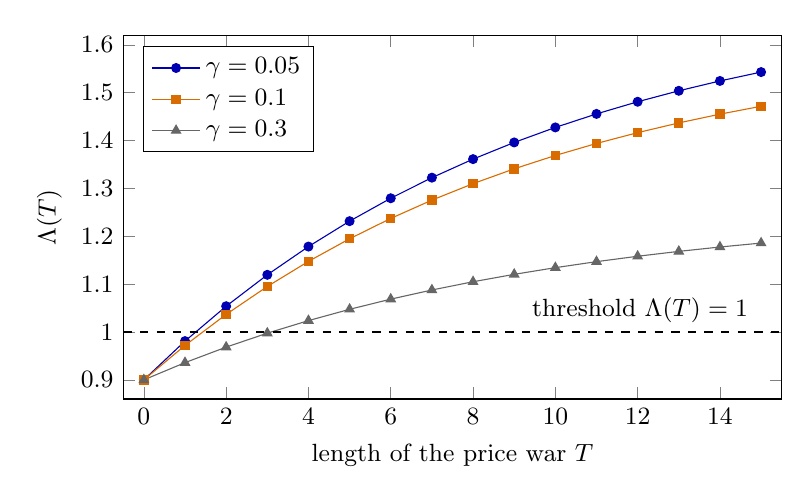
\begin{tikzpicture}
\begin{axis}[
  width=0.82\textwidth, height=6.2cm,
  xlabel={length of the price war $T$}, ylabel={$\Lambda(T)$},
  xmin=-0.5, xmax=15.5, ymin=0.86, ymax=1.62,
  xtick={0,2,4,6,8,10,12,14}, ytick={0.9,1.0,1.1,1.2,1.3,1.4,1.5,1.6},
  legend pos=north west, legend cell align=left,
  tick label style={font=\small}, label style={font=\small}, legend style={font=\small}]
\addplot[blue!70!black, mark=*, mark size=1.6pt, domain=0:15, samples=16]
  {2*(1-0.05)*0.9 + (2*0.05-1)*0.9^(x+1)};
\addlegendentry{$\gamma = 0.05$}
\addplot[orange!85!black, mark=square*, mark size=1.5pt, domain=0:15, samples=16]
  {2*(1-0.1)*0.9 + (2*0.1-1)*0.9^(x+1)};
\addlegendentry{$\gamma = 0.1$}
\addplot[gray!80!black, mark=triangle*, mark size=1.9pt, domain=0:15, samples=16]
  {2*(1-0.3)*0.9 + (2*0.3-1)*0.9^(x+1)};
\addlegendentry{$\gamma = 0.3$}
\addplot[black, dashed, domain=-0.5:15.5, samples=2, forget plot] {1};
\node[font=\small, anchor=south west] at (axis cs:9.2,1.0) {threshold $\Lambda(T) = 1$};
\end{axis}
\end{tikzpicture}
\caption{The left side of the incentive constraint \eqref{eq:12-gp-ic} as a function of the length of the price war,
for $\delta = 0.9$. Collusion is sustainable with punishment length $T$ when $\Lambda(T) \ge 1$. The shortest admissible war
is $T^* = 2$ for $\gamma = 0.05$ and $\gamma = 0.1$, and $T^* = 4$ for $\gamma = 0.3$. The curves approach
$2(1 - \gamma)\delta$ as $T$ grows.}\label{fig:12-gp-ic}
\end{figure}

\begin{figure}[htbp]
\centering
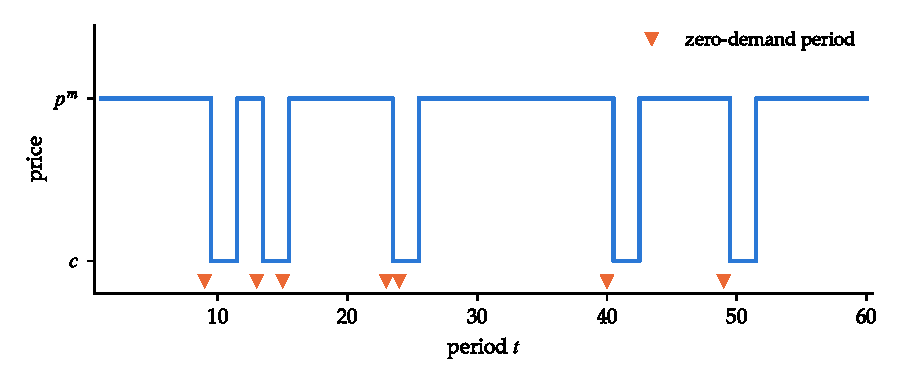
\includegraphics[width=0.92\textwidth]{figures/ch12/gp_path.pdf}
\caption{A simulated equilibrium price path in the Bertrand version of Green and Porter, with $\gamma = 0.1$ and the
optimal war length $T = 2$ for $\delta = 0.9$. Triangles mark periods of zero demand. A zero-demand period in a
collusive phase starts a two-period war at marginal cost. Zero-demand periods inside a war (periods 15 and 24) have
no effect. Wars occupy 10 of the 60 periods, the long-run share $\frac{1}{6}$. Nobody ever cheats. Source: our
simulation, \texttt{figures/ch12/src/gp\_path.py}.}\label{fig:12-gp-path}
\end{figure}

\Cref{fig:12-gp-ic,fig:12-gp-path} summarize four lessons. First, price wars occur on the equilibrium path even
though no firm ever cuts its price. They are necessary: if firms forgave zero sales, undercutting would go
unpunished and collusion would unravel. Second, optimal collusion uses a finite war, as short as the incentive
constraint allows. Third, more noise makes collusion harder. The patience required rises with $\gamma$, and both the
expected collusive profit and the value of collusion fall. Fourth, wars follow unexpectedly low demand. This timing
is the opposite of \cref{sec:12-rs}, where demand is observed and collusive prices are lowest in booms.
\Cref{tab:12-cycle-theories} compares the predictions, and \cref{sec:13-jec} confronts them with data.

The equilibrium has an uncomfortable feature. When a war starts, both firms know that nobody cheated, since each
knows the other's strategy. Both would gain by skipping the war, yet the war is needed to keep conformity optimal in
collusive periods. Equilibria of this kind are not robust to renegotiation after bad outcomes. Cartels that can talk
and audit each other's sales can avoid some of these wars, which is one reason why explicit cartels organize
monitoring (\cref{sec:12-cartels}).

\casehead{N firms, random punishments and the value of transparency}
\Citet[pp.~203--205]{AskerNocke2021} use a variant of this model with $N$ firms and a noisy public signal. It yields
closed forms for the threshold and for the value of collusion, and it shows why transparency matters even far above
the threshold. We state it in our notation. Asker and Nocke write $n$ for $N$, $\beta$ for our $\gamma$, $\alpha$ for
our $\lambda$ and $\rho$ for our $\phi$, and their $\pi^m$ is our expected profit $\bar\pi$.

\begin{assumption}[Bertrand oligopoly with a noisy public signal]\label{asm:12-an}
\leavevmode
\begin{enumerate}[label=(\roman*)]
\item $N$ identical firms sell a homogeneous good at marginal cost $c$. Demand in period $t$ is $\theta_tD(p)$, where
$\theta_t = 0$ with probability $\gamma$ and $\theta_t = 1$ otherwise, independently over time. Write
$\bar\pi = (1 - \gamma)\pi^m$ for the expected monopoly profit.
\item Firms observe neither $\theta_t$ nor rivals' prices. At the start of period $t$ they observe a public signal
$s_t \in \{0, 1\}$. It equals one if some firm priced below $p^m$ in period $t - 1$. If all firms charged at least
$p^m$, it equals one with probability $\lambda$ when $\theta_{t-1} = 0$ and zero otherwise.
\item A public random variable $r_t$, uniform on $[0, 1]$, is drawn at the start of each period. The signal is noisy,
$\gamma\lambda > 0$, and satisfies $\gamma\lambda < \frac{1}{N}$.
\end{enumerate}
\end{assumption}

Under the strategy profile $\sigma(\phi)$, every firm charges $p^m$ until the first period in which $s_t = 1$ and
$r_t \le \phi$. From then on every firm prices at $c$ forever. A bad signal thus triggers Nash reversion with
probability $\phi \in [0, 1]$, and the cartel chooses $\phi$. The profile conditions only on public information. It is
a \emph{perfect public equilibrium} if it is optimal for every firm after every public history.
\Cref{sec:12-abs-repeated} gives the formal definition.

\begin{proposition}[Threshold and value with a noisy signal]\label{prop:12-an}
Under \cref{asm:12-an}, $\sigma(\phi)$ is a perfect public equilibrium if and only if
\begin{equation}\label{eq:12-an-phi}
\phi \;\ge\; \phi^* \equiv \frac{1 - \delta}{\delta}\cdot\frac{N - 1}{1 - N\gamma\lambda} .
\end{equation}
Collusion at $p^m$ is therefore sustainable in this class if and only if
\begin{equation}\label{eq:12-an-delta}
\delta \;\ge\; \underline\delta = \frac{N - 1}{N(1 - \gamma\lambda)} .
\end{equation}
The best such equilibrium uses $\phi^*$, and each firm's per-period value is
\begin{equation}\label{eq:12-an-value}
v^* = (1 - \delta)V(\phi^*) = \frac{1 - N\gamma\lambda}{1 - \gamma\lambda}\cdot\frac{\bar\pi}{N} .
\end{equation}
\end{proposition}

\begin{proof}
On the path, each firm earns $\frac{\bar\pi}{N}$ in expectation. Reversion is triggered next period with probability
$\gamma\lambda\phi$, after which every firm earns zero. The value before reversion therefore solves
\begin{equation*}
V(\phi) = \frac{\bar\pi}{N} + \delta(1 - \gamma\lambda\phi)V(\phi)
\quad\Longrightarrow\quad
V(\phi) = \frac{\bar\pi}{N\bigl[1 - \delta(1 - \gamma\lambda\phi)\bigr]} .
\end{equation*}
A firm that undercuts slightly earns almost $\bar\pi$ in expectation, and the signal then equals one for sure.
Reversion follows with probability $\phi$, so the best one-shot deviation is worth
$V^{\mathrm{dev}}(\phi) = \bar\pi + \delta(1 - \phi)V(\phi)$. Reversion is a stage equilibrium after every history,
so by the one-shot deviation principle the profile is an equilibrium if and only if $V(\phi) \ge V^{\mathrm{dev}}(\phi)$.
Rearrange this as $V(\phi)\bigl[1 - \delta(1 - \phi)\bigr] \ge \bar\pi$ and substitute $V(\phi)$:
\begin{equation*}
\frac{1 - \delta + \delta\phi}{N\bigl[1 - \delta + \delta\gamma\lambda\phi\bigr]} \ge 1
\quad\Longleftrightarrow\quad
1 - \delta + \delta\phi \ge N(1 - \delta) + N\delta\gamma\lambda\phi .
\end{equation*}
Collect the terms in $\phi$:
\begin{equation*}
\delta\phi\,(1 - N\gamma\lambda) \;\ge\; (N - 1)(1 - \delta) .
\end{equation*}
Since $N\gamma\lambda < 1$, dividing gives \eqref{eq:12-an-phi}. A probability $\phi \le 1$ satisfies it if and only
if $\phi^* \le 1$, that is, $\delta(1 - N\gamma\lambda) \ge (N - 1)(1 - \delta)$. Collecting the terms in $\delta$ gives
$\delta(N - N\gamma\lambda) \ge N - 1$, which is \eqref{eq:12-an-delta}. The value $V(\phi)$ falls with $\phi$, so the
best equilibrium in the class uses $\phi^*$. At $\phi^*$,
\begin{equation*}
\delta\gamma\lambda\phi^* = \frac{(1 - \delta)(N - 1)\gamma\lambda}{1 - N\gamma\lambda},
\qquad
1 - \delta + \delta\gamma\lambda\phi^* = (1 - \delta)\,\frac{1 - \gamma\lambda}{1 - N\gamma\lambda} .
\end{equation*}
Substituting into $(1 - \delta)V(\phi^*)$ gives \eqref{eq:12-an-value}.
\end{proof}

These are equations (3) to (5) of Asker and Nocke. Two special cases connect them with the rest of the chapter. With
perfect monitoring, $\lambda = 0$, the threshold is $\frac{N - 1}{N}$ of \cref{prop:12-bertrand} and $v^* =
\frac{\bar\pi}{N}$. With $N = 2$ and $\lambda = 1$, zero demand always triggers the signal, as zero sales do in
\cref{asm:12-gp-bertrand}. The threshold \eqref{eq:12-an-delta} is then $\frac{1}{2(1 - \gamma)}$, the threshold of
\cref{cor:12-gp-optimal-T} for an infinite war.

The result changes how we should read comparative statics. Under perfect monitoring the per-period value jumps from
zero to $\frac{\bar\pi}{N}$ at the threshold and is flat above it. A small change in the number of firms then has no
effect on collusion unless $\delta$ is close to the threshold. With noise, $v^*$ falls continuously with $N$ and with
$\gamma\lambda$ however patient the firms are \citep[p.~205]{AskerNocke2021}. Better observability of deviations, a
lower $\lambda$, lowers the threshold and also raises $v^*$, because the cartel can punish less often on the path.
Take $N = 3$ and $\gamma = 0.2$, our own illustration. With $\lambda = 0.5$ the threshold is
$\frac{2}{3(0.9)} \approx 0.741$ and $v^*$ is $\frac{0.7}{0.9} \approx 0.78$ of the perfect-monitoring value. With
$\lambda = 0.25$ these become $\frac{2}{3(0.95)} \approx 0.702$ and $\frac{0.85}{0.95} \approx 0.89$. This is the
formal content of the view that transparent prices facilitate collusion. \citet{SugayaWolitzky2018} point out a
limit. Some information lets a firm tailor its deviation to current conditions. A cartel member that learns in advance
that its cost of serving a rival's territory is low can deviate exactly then, which makes collusion harder
\citep[p.~205, note~69]{AskerNocke2021}.

\subsection{The original model: Green and Porter (1984)}\label{sec:12-gp-original}

\casehead{Question and context}
\citet{GreenPorter1984} ask how a cartel can enforce collusion when firms cannot observe each other's outputs and
demand is uncertain. Two rigorous formulations of noncooperative collusion existed. In the reaction-function
equilibrium of \citet{Osborne1976}, firms respond to output changes so as to keep their shares. In the supergame of
\citet{Friedman1971}, firms revert to Cournot behavior forever after a price drop. In both, incentives are so perfect
that deterrence is never observed. Time-series data then cannot tell a collusive equilibrium from a competitive one
\citep{Bresnahan1982}. Green and Porter show that this perfection is an artifact of certainty. With imperfect
information, optimal incentive schemes involve recurrent episodes of the conduct previously called price wars or
punishments (pp.~87--88).

\casehead{Which industries the model describes}
The authors list four structural features of a suitable industry (p.~90). First, the industry is stable over time,
which makes rational expectations credible and justifies stationary dynamic programming. Second, output is the only
decision variable. Firms cannot differentiate products or divide the market, so a suspected cheater cannot be
isolated and punished alone. Third, all information except each firm's own output is public. Firms know each other's
cost functions, and all observe a common variable that tells them whether the industry is in a collusive or a
reversionary state. Fourth, this monitoring variable is imperfectly correlated with conduct. Otherwise reversions
would never occur. The fourth feature excludes markets with few, publicly announced transactions, such as contracts
awarded by sealed bids. The authors propose the American rail freight industry of the 1880s as an example
(p.~94), the cartel analyzed by \citet{Porter1983} in \cref{sec:13-jec}.

\begin{assumption}[The Green-Porter environment]\label{asm:12-gp}
\leavevmode
\begin{enumerate}[label=(\roman*)]
\item There are $N$ firms producing a homogeneous good. Firm $i$'s net return from producing $x_i$ units and selling
at price $p$ is $\pi_i(x_i, p)$. Firms are risk neutral and maximize $\E\bigl[\sum_{t \ge 0}\delta^t\pi_i(x_{it}, p_t)\bigr]$.
\item The observed price is
\begin{equation}\label{eq:12-gp-price}
p_t = \eta_t\,P\Bigl(\sum_{i=1}^N x_{it}\Bigr),
\end{equation}
where $P$ is a decreasing inverse demand function and the shocks $\eta_t$ are \iid\ with cdf $F_\eta$, continuous
density $f_\eta$, and $\E[\eta_t] = 1$. No firm observes $\eta_t$.
\item Each firm observes the history of prices and its own outputs. It never observes its rivals' outputs.
\end{enumerate}
\end{assumption}

We change the paper's notation. Its discount factor $\beta$ is our $\delta$, and its inverse demand $p(\cdot)$ is our
$P(\cdot)$. Its demand shock $\theta_t$ is our $\eta_t$, since $\theta$ is the conduct parameter in this book. A
\emph{contingent strategy} for firm $i$ is a sequence $s_i = (s_{i0}, s_{i1}, \dots)$, where $s_{i0}$ is an initial
output and $s_{i,t+1}(p_0, \dots, p_t)$ gives the output at $t + 1$ as a function of past prices. Write $\E_{s}$ for
the expectation under the price process generated by a profile $s$. A \emph{Nash equilibrium} is a profile
$s^* = (s_1^*, \dots, s_N^*)$ such that, for every firm $i$ and every feasible $s_i$ (GP (1), p.~91),
\begin{equation}\label{eq:12-gp-nash}
\E_{s_1^*, \dots, s_i, \dots, s_N^*}\Biggl[\sum_{t = 0}^{\infty}\delta^t\pi_i\bigl(s_{it}(p_0, \dots, p_{t-1}), p_t\bigr)\Biggr]
\;\le\;
\E_{s^*}\Biggl[\sum_{t = 0}^{\infty}\delta^t\pi_i\bigl(s_{it}^*(p_0, \dots, p_{t-1}), p_t\bigr)\Biggr].
\end{equation}

\casehead{Trigger-price strategies}
Let $y = (y_1, \dots, y_N)$ be a profile of \emph{restricted outputs} and $z = (z_1, \dots, z_N)$ the Cournot output
profile of the stage game, in which each firm maximizes its expected one-period return. Fix a \emph{trigger price}
$\bar p$ and an integer $T \ge 2$. Period $t$ is \emph{normal} if (a) $t = 0$, or (b) $t - 1$ was normal and
$p_{t-1} \ge \bar p$, or (c) $t - T$ was normal and $p_{t - T} < \bar p$. Every other period is
\emph{reversionary}. Firm $i$ produces $y_i$ in normal periods and $z_i$ in reversionary periods (pp.~91--92). If a
normal period $t$ ends with $p_t < \bar p$, periods $t + 1, \dots, t + T - 1$ are reversionary and period $t + T$ is
normal again. A reversionary episode therefore lasts $T - 1$ periods, and prices observed during it are ignored. The
length $T$ of the Bertrand version corresponds to $T - 1$ here. The strategies are simple enough to coordinate on,
and Green and Porter suggest that they would arise from an explicit agreement (p.~89, footnote 5).

Each firm faces a stationary dynamic programming problem with $T$ states: normal, and $k$ periods into a reversion
for $k = 1, \dots, T - 1$. In a reversionary period the firm's output does not affect future states, so it maximizes
its expected current return against rivals' Cournot outputs and produces $z_i$. A reversion is thus a temporary
switch to the static Nash equilibrium. In normal periods the problem is the same every time, so the firm's best
policy is a constant output $r$. The question is when $r = y_i$ is optimal.

Let $w_i = \sum_{j \ne i}y_j$ be the rivals' restricted output. Define firm $i$'s expected return in a normal period
when it produces $r$, and its expected Cournot return, as
\begin{equation}\label{eq:12-gp-returns}
\bar\pi_i(r) = \E_\eta\bigl[\pi_i\bigl(r, \eta P(r + w_i)\bigr)\bigr],
\qquad
\pi_i^N = \E_\eta\Bigl[\pi_i\Bigl(z_i, \eta P\Bigl(\sum_j z_j\Bigr)\Bigr)\Bigr]
\end{equation}
(the paper writes $\gamma_i(r)$ and $\delta_i$). Collusion is profitable: $\bar\pi_i(y_i) > \pi_i^N$ for every $i$.
A reversion starts after a normal period in which $\eta P(r + w_i) < \bar p$, an event with probability
\begin{equation}\label{eq:12-gp-Fr}
F_i(r) \equiv \Pr\bigl(\eta P(r + w_i) < \bar p\bigr) = F_\eta\Bigl(\frac{\bar p}{P(r + w_i)}\Bigr).
\end{equation}
This probability rises with $r$, since more output lowers $P(r + w_i)$. Overproduction is detected only
statistically, through a higher chance of a low price.

\begin{proposition}[The value of a trigger-price strategy]\label{prop:12-gp-value}
Under \cref{asm:12-gp}, suppose rivals follow the trigger-price strategies, and firm $i$ produces $r$ in all normal
periods and $z_i$ in all reversionary periods. Let $V_i(r)$ be its expected discounted value in a normal period. Then
(GP (2), p.~92)
\begin{equation}\label{eq:12-gp-bellman}
V_i(r) = \bar\pi_i(r) + \delta\bigl[1 - F_i(r)\bigr]V_i(r) + F_i(r)\Biggl[\sum_{t=1}^{T-1}\delta^t\pi_i^N + \delta^T V_i(r)\Biggr],
\end{equation}
and its solution is (GP (3), p.~92)
\begin{equation}\label{eq:12-gp-value}
V_i(r) = \frac{\pi_i^N}{1 - \delta} + \frac{\bar\pi_i(r) - \pi_i^N}{1 - \delta + (\delta - \delta^T)F_i(r)} .
\end{equation}
\end{proposition}

\begin{proof}
In a normal period the firm earns $\bar\pi_i(r)$ in expectation. With probability $1 - F_i(r)$ the price stays above
$\bar p$, and the next period is normal with value $\delta V_i(r)$. With probability $F_i(r)$ a reversion follows. The
firm earns $\pi_i^N$ in each of the $T - 1$ reversionary periods and returns to a normal period after $T$ periods.
This gives \eqref{eq:12-gp-bellman}. To solve it, use the geometric sum
\begin{equation*}
\sum_{t=1}^{T-1}\delta^t = \frac{\delta - \delta^T}{1 - \delta}
\end{equation*}
and collect the terms in $V_i(r)$:
\begin{equation*}
V_i(r)\bigl[1 - \delta + \delta F_i(r) - \delta^T F_i(r)\bigr] = \bar\pi_i(r) + F_i(r)\,\frac{\delta - \delta^T}{1 - \delta}\,\pi_i^N .
\end{equation*}
Let $\Delta_i(r) \equiv 1 - \delta + (\delta - \delta^T)F_i(r)$ denote the bracket. Then
\begin{equation*}
V_i(r) = \frac{\bar\pi_i(r) + F_i(r)\frac{\delta - \delta^T}{1 - \delta}\pi_i^N}{\Delta_i(r)} .
\end{equation*}
Subtract $\frac{\pi_i^N}{1 - \delta} = \frac{\Delta_i(r)\,\pi_i^N}{(1 - \delta)\Delta_i(r)}$ from both sides. The
numerator on the right becomes
\begin{equation*}
\bar\pi_i(r) + F_i(r)\frac{\delta - \delta^T}{1 - \delta}\pi_i^N - \frac{1 - \delta + (\delta - \delta^T)F_i(r)}{1 - \delta}\pi_i^N
= \bar\pi_i(r) - \pi_i^N ,
\end{equation*}
which gives \eqref{eq:12-gp-value}.
\end{proof}

Equation \eqref{eq:12-gp-value} says that the firm's value equals its value in a permanently Cournot industry plus
the one-period gain from colluding, capitalized at the rate $\Delta_i(r)$. That rate exceeds $1 - \delta$ because
the collusive gain is interrupted by reversions. A larger trigger probability $F_i(r)$ or a longer reversion raises
$\Delta_i(r)$ and lowers the value of collusion.

\casehead{Equilibrium conditions}
The trigger-price profile is a Nash equilibrium if and only if no firm gains by changing its normal-period output
(GP (4), p.~93):
\begin{equation}\label{eq:12-gp-eqm}
V_i(r) \le V_i(y_i) \quad\text{for all } r \text{ and all } i .
\end{equation}
The first-order condition is $V_i'(y_i) = 0$ (GP (5)). The next result writes it out.

\begin{proposition}[The first-order condition]\label{prop:12-gp-foc}
Let $Y = \sum_j y_j$ and $k = \frac{\bar p}{P(Y)}$. At an interior equilibrium, for every $i$ (GP (6), p.~93),
\begin{equation}\label{eq:12-gp-foc}
\bigl[1 - \delta + (\delta - \delta^T)F_\eta(k)\bigr]\,\bar\pi_i'(y_i)
+ (\delta - \delta^T)\,f_\eta(k)\,\frac{\bar p\,P'(Y)}{P(Y)^2}\,\bigl[\bar\pi_i(y_i) - \pi_i^N\bigr] = 0 .
\end{equation}
Equivalently,
\begin{equation}\label{eq:12-gp-foc2}
\underbrace{\bar\pi_i'(y_i)}_{\text{marginal gain}}\;\Delta_i(y_i)
= \underbrace{(\delta - \delta^T)\,f_\eta(k)\,k\,\frac{-P'(Y)}{P(Y)}}_{\text{marginal rise in the risk of reversion}}
\;\underbrace{\bigl[\bar\pi_i(y_i) - \pi_i^N\bigr]}_{\text{loss per period of reversion}} .
\end{equation}
\end{proposition}

\begin{proof}
By \eqref{eq:12-gp-value}, $V_i(r) = \frac{\pi_i^N}{1 - \delta} + \frac{n(r)}{\Delta_i(r)}$ with
$n(r) = \bar\pi_i(r) - \pi_i^N$. Its derivative is zero if and only if $n'(r)\Delta_i(r) - n(r)\Delta_i'(r) = 0$. Here
$n'(r) = \bar\pi_i'(r)$ and, by the chain rule,
\begin{equation*}
\Delta_i'(r) = (\delta - \delta^T)\,f_\eta\Bigl(\frac{\bar p}{P(r + w_i)}\Bigr)\cdot\Bigl(-\frac{\bar p\,P'(r + w_i)}{P(r + w_i)^2}\Bigr).
\end{equation*}
Substituting and evaluating at $r = y_i$, so that $r + w_i = Y$, gives \eqref{eq:12-gp-foc}. Since
$\frac{\bar p}{P(Y)^2} = \frac{k}{P(Y)}$, moving the second term to the right gives \eqref{eq:12-gp-foc2}.
\end{proof}

Equation \eqref{eq:12-gp-foc2} balances two margins (p.~93). The marginal return from producing more in normal
periods is exactly offset by the marginal rise in the risk of a reversion, valued at the loss it causes. Both sides
are positive, since $P' < 0$. Hence $\bar\pi_i'(y_i) > 0$: each firm produces less than its static best
response to its rivals' restricted outputs. The threat of reversion sustains that gap. The $N$ conditions
\eqref{eq:12-gp-foc} restrict the vector $y$, so a given output profile, such as the one that maximizes joint profits,
need not be supportable. A cartel that chooses $(y, \bar p, T)$ to maximize its members' values subject to
\eqref{eq:12-gp-eqm} faces a trade-off. A lower trigger price or a shorter reversion destroys less surplus on the
path but deters less. Green and Porter report that \citet{Porter1983b} solves this problem for symmetric firms. The
optimal normal-period output differs from the monopoly output: firms give up some normal-period profit to reduce the
frequency and duration of reversions (p.~93, footnote 9). The next example illustrates the trade-off.

\begin{example}[A linear duopoly with lognormal shocks]\label{ex:12-gp-linear}
Let $N = 2$, $P(Q) = 1 - Q$, zero marginal cost and $\pi_i(x_i, p) = px_i$. Let
$\ln\eta \sim \mathcal{N}(-\frac{\sigma^2}{2}, \sigma^2)$, so that $\E[\eta] = 1$, with $\sigma = 0.1$ and
$\delta = 0.95$. Each firm's Cournot output is $\frac{1}{3}$ with $\pi_i^N = \frac{1}{9} = 0.1111$, and splitting the
monopoly output gives $y_i = \frac{1}{4}$ with $\bar\pi_i = \frac{1}{8} = 0.125$. With symmetric restricted output
$y$, $\bar\pi_i(r) = r(1 - r - y)$, so $\bar\pi_i'(y) = 1 - 3y$ and $\frac{-P'(Y)}{P(Y)} = \frac{1}{1 - 2y}$. Writing
$u = \frac{1}{\sigma}\bigl(\ln k + \frac{\sigma^2}{2}\bigr)$ in standard units, $F_\eta(k) = \Phi(u)$ and $f_\eta(k)k = \frac{\phi(u)}{\sigma}$,
where $\Phi$ and $\phi$ are the standard normal cdf and density. Condition \eqref{eq:12-gp-foc2} becomes
\begin{equation*}
(1 - 3y)\bigl[1 - \delta + (\delta - \delta^T)\Phi(u)\bigr]
= (\delta - \delta^T)\,\frac{\phi(u)}{\sigma}\;\frac{y(1 - 2y) - \frac{1}{9}}{1 - 2y} .
\end{equation*}
For each $(y, T)$ we solve for the trigger with the smallest reversion probability, check the global condition
\eqref{eq:12-gp-eqm} on a grid of outputs, and compute the normalized value $(1 - \delta)V_i(y)$.
\Cref{tab:12-gp-example} reports the best $y$ for several $T$. Three features stand out. The monopoly split
$y = \frac{1}{4}$ can be supported only with long reversions, $T \ge 14$. For every $T$ the best restricted output
exceeds $\frac{1}{4}$, as in \citet{Porter1983b}: producing more lowers the gain from overproduction and the trigger
probability needed to deter it. Finally, the cartel captures about two thirds of the gain from monopoly over
Cournot, since $\frac{0.1206 - 0.1111}{0.125 - 0.1111} = 0.68$.
\end{example}

\begin{table}[htbp]
\centering
\caption{Best symmetric trigger-price equilibria in the linear duopoly of \cref{ex:12-gp-linear}}\label{tab:12-gp-example}
\begin{tabular}{@{}rccccc@{}}
\toprule
$T$ & Best $y$ & Trigger $\bar p$ & $\Pr(\text{reversion})$ & Long-run share in reversion & $(1 - \delta)V_i$ \\
\midrule
4      & 0.2925 & 0.380 & 0.205 & 0.380 & 0.1177 \\
8      & 0.2800 & 0.380 & 0.079 & 0.357 & 0.1194 \\
16     & 0.2750 & 0.376 & 0.040 & 0.374 & 0.1201 \\
50     & 0.2725 & 0.369 & 0.021 & 0.507 & 0.1205 \\
$\infty$ & 0.2700 & 0.373 & 0.020 & 1     & 0.1206 \\
\midrule
14 ($y = \frac{1}{4}$) & 0.2500 & 0.447 & 0.144 & 0.653 & 0.1171 \\
\bottomrule
\end{tabular}

\smallskip
\begin{minipage}{0.95\textwidth}
\footnotesize Notes: $P(Q) = 1 - Q$, zero cost, $\ln\eta \sim \mathcal{N}(-\frac{\sigma^2}{2}, \sigma^2)$ with
$\sigma = 0.1$, $\delta = 0.95$. Outputs are searched on a grid of step 0.0025 in $[0.20, 0.33]$. Reversions last
$T - 1$ periods. $\Pr(\text{reversion}) = F_\eta(\frac{\bar p}{P(2y)})$ is the probability that a normal period
triggers a reversion. The long-run share of reversionary periods is $\frac{(T-1)G}{1 + (T-1)G}$ with
$G = \Pr(\text{reversion})$ (\cref{prop:12-gp-stationary}). With $T = \infty$ the first reversion is permanent. The
last row is the shortest reversion that supports the monopoly split. With $T = 2$ no output in the grid is an
equilibrium. Benchmarks: Cournot $0.1111$, monopoly split $0.125$. Source: our computation,
\texttt{figures/ch12/src/gp\_design.py}.
\end{minipage}
\end{table}

The example also shows that, in a discounted model, the cartel may prefer an infinite reversion although it ends
collusion for good in the long run. With $\delta = 0.95$, the expected wait of fifty periods before the first
reversion makes its distant cost small. This is a property of the restricted class of trigger strategies with
Cournot reversion. Richer punishments do better, as we discuss below.

\casehead{Properties of the equilibrium}
Two observations complete the formal model (pp.~93--94). First, no firm ever defects. Every firm can compute what
every other firm will produce, so a low price reveals information about demand only. In equilibrium the frequency
of reversions from normal periods is $F_\eta\bigl(\frac{\bar p}{P(\sum_j y_j)}\bigr)$. Second, firms take part in
reversions although they know that low prices reflect demand. A reversion is a temporary switch to a static Nash
equilibrium, so no firm gains by deviating from it unilaterally. If firms ignored low prices and kept colluding, the
first-order condition \eqref{eq:12-gp-foc} would fail in normal periods, and restricted output would no longer be
individually optimal. Green and Porter add that the equilibrium is perfect, citing \citet{Green1980} for a formal
statement (p.~93, footnote 10).

\casehead{A reversal of the traditional interpretation}
The model reverses the traditional reading of a common price pattern (p.~94). Consider an episode in which price
drops sharply, stays low, and then recovers without any cost or demand shock. Such an episode was read as predation
against an entrant, or as the breakdown and re-establishment of a cartel. Either way it signaled fragile collusion. Some
argued that intervention was redundant in markets with such episodes, since the market was already resisting
collusion. In the Green-Porter equilibrium the same episodes are an essential part of a stable collusive scheme. An
industry with the four structural features will show price instability as a stationary feature of collusion. The
policy conclusion is the opposite of the traditional one.

\subsection{The price process and its estimation}\label{sec:12-gp-process}

Because both collusive and reversionary behavior are observed over time, the collusive equilibrium can be
identified statistically. The appendix of \citet{GreenPorter1984} characterizes the price process and shows that its
parameters can be estimated consistently.

\casehead{The switching process}
A \emph{switching process} has four parts (p.~96). The first is a state process $\{W_t\}$ with values in a set $S$
and normal states $S_0 \subset S$. The others are an observed process $\{X_t\}$ and two latent processes $\{Y_t\}$
and $\{Z_t\}$. The
latent variables are independent, the $Y_t$ have a common cdf $G$, the $Z_t$ have a common cdf $H$, and $\{W_t\}$ is
Markov with stationary transition probabilities. The observed variable is $X_t = Y_t$ when $W_t \in S_0$ and
$X_t = Z_t$ otherwise. (In this subsection $G$ and $H$ are local symbols for price distributions.) The usual case has
$S = \{0, 1\}$ and a Bernoulli state process independent of prices.

For the collusive price process, $Y_t$ is the price that would prevail in a normal period and $Z_t$ the price in a
reversionary one. Under \eqref{eq:12-gp-price},
\begin{equation*}
G(p) = F_\eta\Bigl(\frac{p}{P(\sum_j y_j)}\Bigr),
\qquad
H(p) = F_\eta\Bigl(\frac{p}{P(\sum_j z_j)}\Bigr).
\end{equation*}
The states are $S = \{0, 1, \dots, T - 1\}$ with $S_0 = \{0\}$, where state $k \ge 1$ means $k$ periods into a
reversion. The transitions are (GP (A7) to (A10), p.~96)
\begin{equation}\label{eq:12-gp-transitions}
W_{t+1} =
\begin{cases}
0 & \text{if } W_t = 0 \text{ and } Y_t \ge \bar p,\\
1 & \text{if } W_t = 0 \text{ and } Y_t < \bar p,\\
k + 1 & \text{if } W_t = k \text{ with } 1 \le k < T - 1,\\
0 & \text{if } W_t = T - 1 .
\end{cases}
\end{equation}
Since the $Y_t$ are \iid, $\{W_t\}$ is a Markov chain with stationary transition probabilities. Its transition
graph is panel (a) of \cref{fig:12-gp-chain}. Unlike the usual switching model, the state depends on past prices.

\begin{figure}[htbp]
\centering
\begin{subfigure}[b]{0.48\textwidth}
\centering
\begin{tikzpicture}[>=Stealth, st/.style={circle, draw, minimum size=9.5mm, inner sep=0.5pt, font=\small},
  lab/.style={font=\scriptsize}]
\node[st] (s0) at (0,0) {$0$};
\node[st] (s1) at (1.9,-1.4) {$1$};
\node[st] (s2) at (1.9,-3.1) {$2$};
\node[st] (sT2) at (-1.9,-3.1) {$T\!-\!2$};
\node[st] (sT1) at (-1.9,-1.4) {$T\!-\!1$};
\draw[->] (s0) to[loop above] node[lab, above] {$1 - G(\bar p)$} (s0);
\draw[->] (s0) to node[lab, above right] {$G(\bar p)$} (s1);
\draw[->] (s1) to node[lab, right] {$1$} (s2);
\draw[->, dashed] (s2) to[bend left=35] (sT2);
\draw[->] (sT2) to node[lab, left] {$1$} (sT1);
\draw[->] (sT1) to node[lab, above left] {$1$} (s0);
\end{tikzpicture}
\caption{Price process}
\end{subfigure}\hfill
\begin{subfigure}[b]{0.48\textwidth}
\centering
\begin{tikzpicture}[>=Stealth, st/.style={circle, draw, minimum size=9.5mm, inner sep=0.5pt, font=\small},
  lab/.style={font=\scriptsize}]
\node[st] (s0) at (0,0) {$0$};
\node[st] (s1) at (1.9,-1.4) {$1$};
\node[st] (s2) at (1.9,-3.1) {$2$};
\node[st] (sT2) at (-1.9,-3.1) {$T\!-\!2$};
\node[st] (sT1) at (-1.9,-1.4) {$T\!-\!1$};
\draw[->] (s0) to[loop above] node[lab, above] {$1 - G(\bar p)$} (s0);
\draw[->] (s0) to node[lab, above right] {$G(\bar p)$} (s1);
\draw[->] (s1) to node[lab, right] {$1$} (s2);
\draw[->, dashed] (s2) to[bend left=35] (sT2);
\draw[->] (sT2) to node[lab, left] {$1$} (sT1);
\draw[->] (sT1) to node[lab, above left] {$1 - G(\bar p)$} (s0);
\draw[->] (sT1) to node[lab, below] {$G(\bar p)$} (s1);
\end{tikzpicture}
\caption{Approximating process}
\end{subfigure}
\caption{Transition graphs of the state $W_t$. State $0$ is normal, and state $k \ge 1$ is the $k$-th period of a
reversion. In the price process (a), a normal period with a price below $\bar p$ starts a reversion. The
approximating process (b) deletes these triggering periods, so the state leaves $T - 1$ for state $1$ directly when
the next normal price would trigger a reversion. Redrawn from Green and Porter (1984), Figures 1 and 2.}\label{fig:12-gp-chain}
\end{figure}

\casehead{Stationarity and ergodicity}
Green and Porter show that the initial state can be chosen so that $\{X_t\}$ is a stationary ergodic process
(pp.~95--96). Since $X_t$ is a function of $(W_t, Y_t, Z_t)$, it suffices that the joint process is a stationary
Markov process with a unique invariant distribution. A stationary process is \emph{ergodic} if every event that is
unchanged when the time index is shifted has probability zero or one. The \emph{ergodic theorem} then extends the strong law of
large numbers to the process, so sample averages converge to population moments. This is the foundation for the
asymptotic theory of estimators, and it implies that consistent estimators of $\bar p$ and $T$ exist (p.~95).

\begin{proposition}[Stationary distribution of the regimes]\label{prop:12-gp-stationary}
Let $\psi_k$ be the stationary probability of state $k$ under \eqref{eq:12-gp-transitions}. Then
\begin{equation}\label{eq:12-gp-stationary}
\psi_0 = \bigl[1 + (T - 1)G(\bar p)\bigr]^{-1},
\qquad
\psi_k = G(\bar p)\,\psi_0 \quad (k = 1, \dots, T - 1).
\end{equation}
The long-run share of reversionary periods is $\frac{(T - 1)G(\bar p)}{1 + (T - 1)G(\bar p)}$.
\end{proposition}

\begin{proof}
Under the stationary distribution, $\Pr(W_1 = j) = \Pr(W_0 = j) = \psi_j$ for every $j$. For $1 \le k < T - 1$, the
only way to reach state $k + 1$ is from state $k$, with probability one. Hence (GP (A21))
$\psi_{k+1} = \psi_k$. The only way to reach state $1$ is from state $0$ with $Y_0 < \bar p$. Since $Y_0$ is
independent of $W_0$, this gives (GP (A22)) $\psi_1 = \psi_0 G(\bar p)$. So $\psi_k = G(\bar p)\psi_0$ for
$k = 1, \dots, T - 1$. The probabilities sum to one:
\begin{equation*}
\psi_0 + (T - 1)G(\bar p)\psi_0 = 1 ,
\end{equation*}
which gives (GP (A23)) the first formula. The share of reversionary periods is $1 - \psi_0$.
\end{proof}

The share formula matches \eqref{eq:12-gp-war-share} with $\gamma$ replaced by $G(\bar p)$ and $T$ by $T - 1$. In
equilibrium $G(\bar p) = F_\eta(\frac{\bar p}{P(\sum_j y_j)})$, the frequency of reversions noted above.

\casehead{The approximating process and contamination}
Maximum likelihood estimation of the price process is awkward, because the regime depends on past prices.
\Citet{Porter1983} instead estimates a related process that keeps the dependence of the regime on its own past but
makes the regime independent of prices (p.~97). This \emph{approximating process} has three properties. Normal
prices are drawn from the distribution of $Y$ conditional on $Y \ge \bar p$ (GP (A11)),
\begin{equation*}
J(p) = \max\Bigl[\frac{G(p) - G(\bar p)}{1 - G(\bar p)},\, 0\Bigr].
\end{equation*}
The regime, normal prices and reversionary prices are mutually independent (GP (A12)). The regime is a stationary
Markov chain with the transitions in panel (b) of \cref{fig:12-gp-chain} (GP (A13)). The advantage is that existing
work on the maximum likelihood estimation of switching processes applies. The estimator is cheap to compute, and
results on its consistency and asymptotic normality are available (p.~97).

The approximating process is obtained from the price process by deleting the triggering observations, the normal
periods in which $Y_t < \bar p$ (pp.~97--98). A \emph{stopping time} is a random date whose occurrence is determined
by the history up to that date. Formally, define stopping times by $\tau_0 = 1$ if $W_0 = 0$ and $Y_0 < \bar p$,
$\tau_0 = 0$ otherwise, and
\begin{equation*}
\tau_{t+1} =
\begin{cases}
\tau_t + 2 & \text{if } W_{\tau_t + 1} = 0 \text{ and } Y_{\tau_t + 1} < \bar p,\\
\tau_t + 1 & \text{otherwise.}
\end{cases}
\end{equation*}
We set $X_t' = X_{\tau_t}$ and re-index the state and latent variables in the same way (GP (A14) to (A17)). Because
the chain restarts afresh at each such date (the \emph{strong Markov property}), the censored state process is a
stationary Markov chain, now independent of prices.
Conversely, the observed price series is a \emph{contaminated} sample path of the approximating process. The
contaminating observations are the triggering prices, which the approximating process does not contain.

\begin{proposition}[The contamination ratio]\label{prop:12-gp-contamination}
With probability one (GP (A24), p.~99),
\begin{equation}\label{eq:12-gp-contamination}
\lim_{t \to \infty}\frac{\tau_t - t}{\tau_t} = \frac{G(\bar p)}{1 + (T - 1)G(\bar p)} .
\end{equation}
\end{proposition}

\begin{proof}
Let $a(W, Y) = 1$ if $W = 0$ and $Y < \bar p$, and $a(W, Y) = 0$ otherwise. Each deleted observation is a period
with $a = 1$, so $\tau_t = t + \sum_{u=0}^{\tau_t}a(W_u, Y_u)$ and (GP (A18))
\begin{equation*}
\frac{\tau_t - t}{\tau_t} = \frac{1}{\tau_t}\sum_{u=0}^{\tau_t}a(W_u, Y_u) .
\end{equation*}
By the ergodic theorem the average converges almost surely to $\Pr(W_0 = 0, Y_0 < \bar p)$ (GP (A19)). The state
$W_0$ depends only on draws before period 0, and the $Y_t$ are \iid. Hence $W_0$ and $Y_0$ are independent, and the
limit is $\psi_0 G(\bar p)$ (GP (A20)). Substituting $\psi_0$ from
\cref{prop:12-gp-stationary} gives \eqref{eq:12-gp-contamination}.
\end{proof}

\begin{table}[htbp]
\centering
\caption{Green and Porter's illustration of the contamination of the approximating process}\label{tab:12-gp-contamination}
\begin{tabular}{@{}lll@{}}
\toprule
Quantity & Formula & Value \\
\midrule
Probability that a normal week triggers a reversion & $G(\bar p)$ & 0.025 \\
Length of a reversion (weeks) & $T - 1$ & 10 \\
Expected length of a normal episode (weeks) & $\frac{1}{G(\bar p)}$ & 40 \\
Long-run share of normal weeks & $\psi_0 = [1 + (T - 1)G(\bar p)]^{-1}$ & $\frac{1}{1.25} = 0.8$ \\
Contamination ratio & $\psi_0 G(\bar p)$ & $\frac{0.025}{1.25} = 0.02$ \\
\midrule
\multicolumn{3}{@{}l}{Contamination of each subsample used by the estimator} \\
\quad Triggering prices split proportionally & & 2 percent \\
\quad All triggering prices in the normal subsample & $\frac{0.02}{0.8}$ & 2.5 percent \\
\quad All triggering prices in the reversionary subsample & $\frac{0.02}{0.2}$ & 10 percent \\
\bottomrule
\end{tabular}

\smallskip
\begin{minipage}{0.95\textwidth}
\footnotesize Notes: A period is one week, as when a trade association circulates weekly prices. The parameter values
$G(\bar p) = 0.025$ and $T = 11$ and the contamination levels are those of the example in \citet[p.~99]{GreenPorter1984}.
The intermediate quantities are computed from \cref{prop:12-gp-stationary,prop:12-gp-contamination}.
\end{minipage}
\end{table}

\Cref{tab:12-gp-contamination} reproduces the authors' numerical illustration (p.~99). With weekly data,
$G(\bar p) = 0.025$ and $T = 11$, a normal episode lasts forty weeks on average and a reversion ten weeks. A
reversion therefore occurs about once a year, and about one price observation a year is a triggering price that the
approximating process would not contain. The contamination ratio is one in fifty. The estimator splits the sample
into a subsample attributed to $G$ and one attributed to $H$, and estimates each distribution separately. If the
contaminating observations were spread in proportion, each subsample would be 2 percent contaminated. If all of them
were assigned to the normal subsample, its contamination would be 2.5 percent, which still seems negligible. If all
of them were assigned to the reversionary subsample, which is only one fifth of the data, its contamination would be
10 percent. In this worst case the low draws from $G$ could bias the estimate of $H$ seriously. Green and Porter
note that these parameter values are approximately those that \citet{Porter1983} reports for the rail freight
cartel. They conclude that the bias is plausibly slight under optimistic assumptions, while acknowledging an element
of judgment (p.~99). \Cref{sec:13-implications,sec:13-jec} develop the estimator and Porter's results.

\subsection{Testable implications, extensions and critiques}\label{sec:12-gp-assessment}

\casehead{Testable implications}
The model makes several predictions that distinguish it from collusion under perfect monitoring. Conduct switches
between discrete regimes, so the supply relation shifts between a collusive and a Cournot (or Bertrand) regime.
Reversions start after unexpectedly low prices, which reflect unobserved negative demand shocks rather than
observable booms. Reversions have a fixed and finite length in the simplest version. In normal periods output
exceeds the joint-profit level when the cartel designs its scheme optimally. \Cref{ch:collusion-evidence} tests these
predictions with the data of the Joint Executive Committee and compares them with those of
\cref{sec:12-demand} (\cref{sec:13-jec,sec:13-implications}). The regime switches also imply that a single conduct
parameter estimated over the whole sample averages two conducts, the problem discussed in \cref{ch:conduct}.

\casehead{Extensions}
Green and Porter study only the simplest trigger-price strategies. Firms might, for example, condition the length of
a reversion on how far the price falls below $\bar p$ (p.~92, footnote 8). \Citet{Porter1983b} chooses the trigger
price, the reversion length and the restricted output optimally. \Citet{AbreuPearceStacchetti1986} characterize
optimal symmetric equilibria of a Green-Porter industry without restricting strategies. We follow the account of
\citet[section~6.7.1.2]{Tirole1988}. Two assumptions give sharp results. First, the firms' payoff functions are
concave. Second, the distribution of the market price given aggregate output satisfies the \emph{monotone likelihood
ratio property} (MLRP). Informally, a low price is more likely to come from a high output than from a low one. Under these
assumptions, attention can be restricted to two phases with values $V^+$ and $V^-$, the best and the worst payoffs in
the set of symmetric perfect equilibria. In the collusive phase each firm produces $q^+$, and a punishment starts if
the price falls below a threshold $p^+$. This \emph{tail test} is the trigger of \citet{GreenPorter1984}. The
punishment phase has no fixed length. Each firm produces a high output $q^-$. Play stays in the punishment phase as
long as the price exceeds a second threshold $p^-$, and it returns to the collusive phase when the price falls below
$p^-$. This \emph{inverse tail test} looks odd at first. A harsh punishment requires an output higher than each firm
would choose privately. A high price signals low output, so it is a high price that prolongs the punishment. The
two phases follow a Markov process, and punishments can be harsher than Cournot reversion. \Citet{AbreuPearceStacchetti1990} develop the recursive method behind this result (\cref{sec:12-aps}).
\Citet{FudenbergLevineMaskin1994} give conditions on how the distribution of the public signal responds to each
player's actions under which a folk theorem holds with imperfect public monitoring. When signals are private to each
firm, as with secret sales, the problem is harder, and \cref{sec:12-hs} studies how cartels solve it with reports and
transfers.

\casehead{Critiques}
Several limitations qualify the model. First, the restriction to trigger strategies with Cournot reversion is not
innocuous: as noted above, richer punishments do better. Second, wars are costly to the cartel, and firms that know
nobody cheated have a reason to renegotiate them away. Third, the source of the inference problem matters.
\Cref{sec:12-private-costs} shows that when firms have private information about costs and prices are public, optimal
collusion typically needs no wars at all. Fourth, real cartels communicate, exchange sales data and make transfers,
which changes the monitoring problem (\cref{sec:12-cartels}). Fifth, \citet{LevensteinSuslow2006} find that many price
wars in documented cartels arise from bargaining over shares rather than from noise (\cref{sec:12-success}). Sixth, the
shocks are \iid. Green and Porter note that a martingale specification would suit durable goods better and accept
that the \iid\ assumption is restrictive (p.~91, footnote 7). Finally, the four structural conditions are demanding,
and the authors concede that the direct applicability of the model is severely limited (p.~94).

\casehead{Contribution}
\citet{GreenPorter1984} provided the first equilibrium theory of price wars as part of a working cartel. They turned
Stigler's policing problem into a repeated game with imperfect public monitoring, reversed the received reading of
price instability, and showed that the resulting price process can be estimated. The paper set the template for the
theory of repeated games with imperfect monitoring and, through \citet{Porter1983}, for the empirical study of
cartel regimes in \cref{ch:collusion-evidence}.

\section{Private Information about Costs: Collusion and Price Rigidity}\label{sec:12-private-costs}

The models so far share one feature: firms are identical in every period. In practice each firm's costs move with
input prices, breakdowns and the quality of its own operations, and rivals do not observe them. A cartel that wants
the lowest-cost firm to serve the market must then learn who has low costs, and firms have an incentive to lie. This
section studies \citet{AtheyBagwellSanchirico2004}, abbreviated ABS, who analyze collusion when prices are public and
costs are private. We work from the November 1998 working-paper version. Page and result numbers refer to it and may
differ from the published article.

\subsection{Question and motivation}\label{sec:12-abs-question}

ABS place their model as the third canonical extension of the standard collusion model (pp.~1--2). In
\citet{RotembergSaloner1986}, demand shocks are public and collusive prices vary with them, without wars on the
path (\cref{sec:12-rs}). In \citet{GreenPorter1984}, actions are hidden and wars follow bad shocks. This is a model of
repeated \emph{moral hazard}, or hidden action. ABS study repeated \emph{adverse selection}, or hidden information:
each firm privately observes its cost, while prices are observed by all.

The application is the relation between collusion and price rigidity. Empirical studies going back to the 1920s,
including \citet{Carlton1986,Carlton1989}, find that prices are more rigid in concentrated industries (p.~2).
\citet{Scherer1980} summarizes studies in which collusion is implemented by rules of thumb, such as a fixed
percentage above a common wholesale price. The price then ignores members' private cost positions. The best-known
theory of rigidity is the kinked demand curve \citep{Sweezy1939,HallHitch1939}, which assumes that rivals match price
cuts but not increases. As ABS note, it rests on an ad hoc behavioral postulate, compresses a dynamic story into a
static model, and does not determine the price. Economists therefore fell back on an informal view.
\citet[pp.~914--915]{Carlton1989} states it as follows: ``Anytime a price change occurs in an oligopoly, there is a risk
that a price war could break out. Hence, firms are reluctant to change price.'' ABS give this view a rigorous form.

\citet[section~6.2.1]{Tirole1988} spells out the static story and its weakness. Each of two firms with cost $c$
conjectures that its rival will match any cut below a \emph{focal price} $p^f$ and will ignore any increase. A firm's
perceived demand is then $\frac{D(p)}{2}$ below $p^f$ and zero above it. If $(p - c)D(p)$ is quasi-concave, the best
price under this conjecture is $p^f$ when $p^f \le p^m$. Every focal price between $c$ and $p^m$ is therefore
consistent with the conjectures. The story explains too much, and it says nothing about how the focal price responds
to a change in cost. \citet{MaskinTirole1988} give the kinked demand curve an equilibrium foundation. Firms set prices
in alternate periods and keep each price for two periods, so a firm's current price affects its rival's profit. In a
\emph{Markov perfect equilibrium}, each firm's price depends only on the rival's current price. One such equilibrium
has a focal price at the monopoly level. A firm that raises its price is not followed, and a firm that undercuts
provokes a price war, after which the firms eventually return to the focal price \citep[section~6.4.1]{Tirole1988}. Tirole
reports two further results (section~6.4.2). Industry profit in every Markov perfect equilibrium is bounded away from
zero. For discount factors close to one, the average profit in a symmetric equilibrium is at least half the monopoly
profit. Other Markov equilibria never settle and produce cycles of price wars and relenting, the Edgeworth
cycles of \cref{sec:13-noel}. Retaliation in this model has a tangible motive, unlike the bootstrap strategies of
\cref{sec:12-finite}. ABS reach rigidity by a different route. In their model a rigid price is the cheapest way to
collude when costs are private, whereas in Maskin and Tirole it follows from short-run commitment to prices.

\subsection{The static game}\label{sec:12-abs-static}

\begin{assumption}[The ABS stage game]\label{asm:12-abs}
\leavevmode
\begin{enumerate}[label=(\roman*)]
\item $N \ge 2$ firms compete in prices in a homogeneous-good market (ABS write $n$).
\item Firm $i$'s unit cost $c_i$ is its private information. Costs are \iid\ across firms with cdf $F$ on
$[\underline c, \bar c]$ and a density $f$ that is positive everywhere (ABS write $\theta$ for the cost).
\item A unit mass of identical consumers has demand $D(p)$. Demand is either \emph{inelastic}, with $D(p) = 1$ for
$p \le \bar v$ and zero above, where the reservation value satisfies $\bar v \ge \bar c$ (ABS write $r$), or
\emph{downward sloping}: positive, twice continuously differentiable and decreasing.
\item The profit of a firm that serves the whole market, $\pi(p, c) = (p - c)D(p)$, is strictly quasi-concave in $p$
with a unique maximizer $p^m(c)$.
\item The lowest price wins, and ties are split equally.
\end{enumerate}
\end{assumption}

Under inelastic demand $p^m(c) = \bar v$ for every $c$, and the game is a first-price procurement auction. With
downward-sloping demand $p^m(c)$ increases with $c$. A \emph{pricing schedule} $p_i(c)$ maps costs into prices, and
is continuously differentiable except at finitely many points, so that jumps are allowed. Let
$\mathbf{p} = (p_1, \dots, p_N)$ be a vector of realized prices. Firm $i$'s market share $m_i(\mathbf p)$ equals one
if $p_i$ is strictly lowest, $\frac{1}{k}$ if $p_i$ ties with $k - 1$ rivals for the lowest price, and zero otherwise.
Its \emph{interim profit}, the expected profit given its cost $c_i$ and price $p_i$ when rivals use schedules
$p_{-i}(\cdot)$, is
\begin{equation}\label{eq:12-abs-interim}
\Pi_i\bigl(p_i, p_{-i}, c_i\bigr) = \pi(p_i, c_i)\;\E\bigl[m_i\bigl(p_i, p_{-i}(c_{-i})\bigr)\bigr],
\end{equation}
where the expectation is over the rivals' costs. The product form shows the trade-off. A lower price reduces the
profit if the firm wins but raises the probability of winning.

Firms of different types weigh this trade-off differently. The cross-partial derivatives satisfy
\begin{equation}\label{eq:12-abs-sc}
\pi_c(p, c) = -D(p) < 0,
\qquad
\pi_{pc}(p, c) = -D'(p) \ge 0 ,
\end{equation}
with strict inequality under downward-sloping demand. A lower-cost firm earns more if it wins, so it values the
extra chance of winning more. A price cut also reduces its profit-if-win by less, because its extra units cost less.
This is a \emph{single-crossing property}: lower types find a price cut more attractive than higher types. As in
mechanism design, it implies that equilibrium schedules are non-decreasing in cost.

\begin{proposition}[The static equilibrium, \citealp{Spulber1995}]\label{prop:12-abs-static}
Under \cref{asm:12-abs}, the static game has a unique Nash equilibrium (ABS Proposition 1, p.~10). It is symmetric,
$p_i = p^e$ for all $i$. The schedule $p^e$ is continuously differentiable and strictly increasing on
$(\underline c, \bar c)$ and lies below the monopoly price, $p^e(c) < p^m(c)$ for $c < \bar c$. Every type except
$\bar c$ earns a positive interim profit, and $p^e(\bar c) = \bar c$.
\end{proposition}

Under inelastic demand the equilibrium is the low-bid equilibrium of \cref{prop:14-proc-bid}. A firm with cost $c$
wins when all $N - 1$ rivals have higher costs, an event with probability $[1 - F(c)]^{N-1}$, and
\begin{equation}\label{eq:12-abs-pe}
p^e(c) = c + \frac{\int_c^{\bar c}[1 - F(t)]^{N-1}\,dt}{[1 - F(c)]^{N-1}} .
\end{equation}

\begin{example}[Uniform costs]\label{ex:12-abs-static-uniform}
Let costs be uniform on $[0, 1]$ and $\bar v = 1$. Then $[1 - F(t)]^{N-1} = (1 - t)^{N-1}$ and
$\int_c^1(1 - t)^{N-1}dt = \frac{(1 - c)^N}{N}$, so
\begin{equation*}
p^e(c) = c + \frac{1 - c}{N} .
\end{equation*}
Type $c$ earns the interim profit $(p^e(c) - c)(1 - c)^{N-1} = \frac{(1 - c)^N}{N}$, and the ex ante profit per firm
is
\begin{equation*}
\int_0^1\frac{(1 - c)^N}{N}\,dc = \frac{1}{N(N + 1)} .
\end{equation*}
With two firms, $p^e(c) = \frac{1 + c}{2}$, interim profit is $\frac{(1 - c)^2}{2}$, and ex ante profit is
$\frac{1}{6}$. If instead both firms always charged $\bar v = 1$ and split the market, each would earn
$\frac{1 - \E c}{2} = \frac{1}{4}$ per period. This rigid price gives up efficiency but raises profit by half.
\end{example}

The static equilibrium has no flat segments and no jumps (p.~10). If the schedule jumped up at $\hat c$, a firm of
type $\hat c$ would raise its price into the gap without losing any sales. If the schedule were flat on an interval,
a firm on it would shade its price slightly and turn ties into wins. These arguments rely on the winner-take-all
nature of the one-shot game, and they fail in the repeated game.

\subsection{The repeated game and its recursive formulation}\label{sec:12-abs-repeated}

\casehead{Information and strategies}
Firms play the stage game in every period. Costs are drawn independently across firms and periods. At the start of
a period a firm knows its own past costs and schedules and the realized prices of all firms, but not its rivals' costs
or schedules (pp.~10--11). A \emph{public strategy} conditions only on the history of realized prices. A
\emph{sequential equilibrium} specifies strategies and beliefs about rivals' private information. Each player's
strategy must be optimal after every history given its beliefs, and beliefs must follow Bayes' rule wherever possible.
A perfect public equilibrium (PPE) is a profile of public strategies that is a sequential equilibrium. It is
immune to deviations that condition on private histories \citep{FudenbergLevineMaskin1994}. Because costs are \iid,
the continuation of a PPE after any public history is itself a PPE (ABS Lemma 2, p.~11).

\begin{definition}[Symmetric perfect public equilibrium]\label{def:12-sppe}
A PPE is a \emph{symmetric perfect public equilibrium} (SPPE) if after every public history all firms use the same
pricing schedule.
\end{definition}

Symmetry means that firms share punishments and rewards. A firm that keeps charging implausibly low prices risks an
industry-wide breakdown, which is the ``fear of breakdown'' of the informal literature (p.~12). Symmetric schemes are
also the only option when firms see the prices offered without knowing who offered them. Procurement auctions with
more than two bidders that announce the winning bid, but not the name of the winner, are an example (p.~7).

\casehead{Two kinds of deviations}
A collusive scheme must deter two kinds of deviations (p.~11). An \emph{off-schedule} deviation is a price that no
type is supposed to charge. It reveals a deviation for sure, so a punishment can follow, and if the punishment
deters it the punishment never occurs. An \emph{on-schedule} deviation is a price assigned to another type, typically
a lower price assigned to a lower cost. Rivals cannot tell it from truthful behavior. Deterring it with a punishment
after low prices is costly, because the punishment then occurs on the path whenever costs are truly low.

The repeated game also allows schedules that the static game rules out (p.~12). A flat schedule can be supported if
undercutting it triggers a war. Lowering one's price now changes three things: the chance of winning, the
profit-if-win, and the continuation value. The mix of the two incentive problems is chosen by the firms. A fully flat
schedule has an acute off-schedule problem and no on-schedule problem. A schedule that spans all relevant prices has
no off-schedule problem but possibly an acute on-schedule problem. By choosing the schedule, firms choose the support
of the public signal.

\casehead{The Factored Program}
Let $\Pi(p)$ be a firm's ex ante profit when all firms use schedule $p$, and $\Pi(p', p)$ its profit when it uses
$p'$ and its rivals use $p$. Let $\mathcal V$ be the set of SPPE continuation values, with supremum $\bar{\mathcal V}$.
A symmetric public profile can be factored into a first-period schedule $p$ and a continuation function
$v: \R_+^N \to \R$ that gives the common continuation value after each vector of first-period prices. Each firm's
payoff is $\Pi(p) + \delta\E v(\mathbf p)$, where $\mathbf p$ is the random price vector generated by $p$. ABS
consider the following problem (p.~13):
\begin{equation}\label{eq:12-abs-factored}
\begin{aligned}
\max_{p,\,v}\quad & \Pi(p) + \delta\E v(\mathbf p)\\
\text{s.t.}\quad & v(\mathbf p) \in \mathcal V \quad\text{for all } \mathbf p \in \R_+^N,\\
& \Pi(p) + \delta\E v(\mathbf p) \ge \Pi(p', p) + \delta\E v(p', p) \quad\text{for all } p' .
\end{aligned}
\end{equation}

\begin{lemma}[Factorization]\label{lem:12-abs-factor}
If a symmetric public profile factors into $(p^*, v^*)$ and $(p^*, v^*)$ solves \eqref{eq:12-abs-factored}, the
profile is an optimal SPPE (ABS Lemma 3, p.~13).
\end{lemma}

The lemma follows because $(p, v)$ is the factorization of some SPPE if and only if it satisfies the two constraints.
Every SPPE has continuation values in $\mathcal V$ by the recursion property, and it must be immune to deviations in
the first period. Conversely, appending to $p$ the SPPE continuations that deliver $v(\mathbf p)$ yields a profile
that is an SPPE by the one-shot deviation principle. This is the self-generation logic of
\citet{AbreuPearceStacchetti1990} described in \cref{sec:12-aps}.

\casehead{The Interim Program}
Splitting the incentive constraint by type and by kind of deviation gives an equivalent problem (p.~14). Let
$\E_{-i}$ denote the expectation over rivals' costs when rivals use $p$, and write $v(p_i, \mathbf p_{-i})$ for the
continuation value after firm $i$ charges $p_i$ and rivals charge $\mathbf p_{-i}$. The firms choose $p$ and $v$ to
maximize $\E_c\bigl[\Pi(p(c), p, c) + \delta\E_{-i}v(p(c), \mathbf p_{-i})\bigr]$ subject to two sets of
constraints. The \emph{off-schedule constraints} must hold for every price $p' \notin p([\underline c, \bar c])$:
\begin{align}
& v(p', \mathbf p_{-i}) \in \mathcal V \ \text{ for all } \mathbf p_{-i}, \tag{IC-off1}\label{eq:12-ic-off1}\\
& \Pi(p(c), p, c) + \delta\E_{-i}v(p(c), \mathbf p_{-i}) \ge \Pi(p', p, c) + \delta\E_{-i}v(p', \mathbf p_{-i})
\ \text{ for all } c. \tag{IC-off2}\label{eq:12-ic-off2}
\end{align}
The \emph{on-schedule constraints} must hold for every announced type $\hat c$:
\begin{align}
& v(p(\hat c), \mathbf p_{-i}) \in \mathcal V \ \text{ for all } \mathbf p_{-i}, \tag{IC-on1}\label{eq:12-ic-on1}\\
& \Pi(p(c), p, c) + \delta\E_{-i}v(p(c), \mathbf p_{-i}) \ge \Pi(p(\hat c), p, c) + \delta\E_{-i}v(p(\hat c), \mathbf p_{-i})
\ \text{ for all } c . \tag{IC-on2}\label{eq:12-ic-on2}
\end{align}
The on-schedule constraint \eqref{eq:12-ic-on2} is written in direct form. A firm of type $c$ must prefer the price of
its own type to the price of any other type $\hat c$, as in a truth-telling constraint.

\casehead{The Mechanism Design Program}
Define a firm's interim profit when its true cost is $c$ and it charges the price of type $\hat c$:
\begin{equation}\label{eq:12-abs-U}
U(\hat c, c; p) \equiv \Pi\bigl(p(\hat c), p, c\bigr) = \pi\bigl(p(\hat c), c\bigr)\,M(\hat c; p),
\qquad
M(\hat c; p) \equiv \E_{-i}\bigl[m_i\bigl(p(\hat c), \mathbf p_{-i}\bigr)\bigr].
\end{equation}
Here $M(\hat c; p)$ is the expected market share of a firm that charges $p(\hat c)$, and ABS write $H$ for $U$. Define
the expected \emph{war} that follows the price of type $c$,
\begin{equation}\label{eq:12-abs-T}
\mathcal T(c) \equiv \delta\bigl[\bar{\mathcal V} - \E_{-i}v\bigl(p(c), \mathbf p_{-i}\bigr)\bigr] \ge 0 ,
\end{equation}
the discounted shortfall of the continuation value below its supremum (ABS write $T$). The \emph{Mechanism Design
Program} (p.~15) is
\begin{equation}\label{eq:12-abs-mdp}
\max_{p,\,\mathcal T}\;\E\bigl[U(c, c; p) - \mathcal T(c)\bigr]
\quad\text{s.t.}\quad
\mathcal T(c) \ge 0 \text{ for all } c,
\end{equation}
\begin{equation*}\tag{IC-onM}\label{eq:12-ic-onM}
U(c, c; p) - \mathcal T(c) \ge U(\hat c, c; p) - \mathcal T(\hat c) \quad\text{for all } c, \hat c .
\end{equation*}
Since $\E[U - \mathcal T] = \E[\Pi(p(c), p, c) + \delta\E_{-i}v] - \delta\bar{\mathcal V}$, the objective is that of
the Interim Program up to a constant. Any $(p, v)$ that satisfies the Interim Program's constraints maps through
\eqref{eq:12-abs-T} into a pair $(p, \mathcal T)$ that satisfies \eqref{eq:12-ic-onM}, with $\mathcal T \ge 0$
because $v \le \bar{\mathcal V}$. The Mechanism Design Program is therefore a relaxation. It drops the off-schedule
constraints, which patient firms can satisfy, and the requirement that the wars be implementable by continuation
values in $\mathcal V$.

\Cref{tab:12-abs-analogy} records the analogy with static mechanism design (pp.~3--4, 42). The analogy has a twist.
In a standard principal-agent problem a principal extracts rents from the agent, and incentive compatibility puts a
lower bound on the agent's profit. Here the agents design their own scheme to maximize their joint profit, and
incentive compatibility puts an upper bound on what each type can be given (p.~17).

\begin{table}[htbp]
\centering
\caption{Collusion with private costs as a mechanism design problem}\label{tab:12-abs-analogy}
\begin{tabularx}{\textwidth}{@{}>{\raggedright\arraybackslash}X>{\raggedright\arraybackslash}X>{\raggedright\arraybackslash}X@{}}
\toprule
Repeated game & Static mechanism design & Difference \\
\midrule
On-schedule constraint (no type mimics another) & Incentive compatibility (truth-telling) & None \\
Off-schedule constraint (no type undercuts the schedule) & Participation constraint & The outside option depends on the type, the schedule and the future value of collusion \\
Continuation values after each price vector & Transfers & Restricted: a war is borne by all firms, is wasteful, and cannot be negative (no subsidies, $\mathcal T \ge 0$) \\
Pricing schedule $p(c)$ & Allocation rule & The allocation $M(c; p)$ is induced by prices and the tie rule \\
\bottomrule
\end{tabularx}

\smallskip
\begin{minipage}{0.95\textwidth}
\footnotesize Notes: Based on \citet{AtheyBagwellSanchirico2004}, working-paper version, pp.~3--4, 14--15 and 41--43.
Asymmetric equilibria (\cref{sec:12-abs-asymmetric}) also allow transfers from one firm to another.
\end{minipage}
\end{table}

\begin{proposition}[Staticizing]\label{prop:12-abs-staticizing}
Suppose the Mechanism Design Program is solved by $(p^*, \mathcal T^*)$ with $\mathcal T^* \equiv 0$. Then there is
$\delta_0 \in (0,1)$ such that, for $\delta \ge \delta_0$ (ABS Proposition 4, p.~16):
\begin{enumerate}[label=(\roman*)]
\item The schedule $p^*$ maximizes $\E U(c, c; p)$ subject to $U(c, c; p) \ge U(\hat c, c; p)$ for all $c, \hat c$.
\item In an optimal SPPE, firms use $p^*$ after all equilibrium-path histories.
\item The best SPPE value is $\bar{\mathcal V} = \frac{\E U(c, c; p^*)}{1 - \delta}$, and it belongs to $\mathcal V$.
\end{enumerate}
\end{proposition}

The argument is as follows (pp.~15--16). Replace the requirement $v \in \mathcal V$ by $v \in \mathcal V \cup
\{\bar{\mathcal V}\}$ in the Interim Program. Setting $v \equiv \bar{\mathcal V}$ after all on-schedule prices solves
the relaxed problem, so $\E U(c, c; p^*) + \delta\bar{\mathcal V} \ge \bar{\mathcal V}$, that is,
$\frac{\E U(c, c; p^*)}{1 - \delta} \ge \bar{\mathcal V}$. Since $\mathcal T^* \equiv 0$, the schedule $p^*$
satisfies the on-schedule constraints with any continuation that does not vary across types. Repeating $p^*$ forever,
with reversion to the static Nash equilibrium after off-schedule prices, is then an SPPE for patient firms, as long as
$p^*$ beats static Nash profits. Its value $\frac{\E U(c, c; p^*)}{1 - \delta}$ lies in $\mathcal V$ and therefore
equals $\bar{\mathcal V}$. The problem of finding an optimal SPPE thus reduces to a static mechanism design problem.
The rest of the analysis asks when the solution has no wars.

\subsection{Incentive compatibility and efficiency rents}\label{sec:12-abs-ic}

Write $Q(c; p) \equiv D(p(c))M(c; p)$ for the expected quantity sold by type $c$. Since $U(\hat c, c; p) = (p(\hat c) -
c)D(p(\hat c))M(\hat c; p)$ is affine in the true cost $c$, its derivative with respect to $c$ is
\begin{equation}\label{eq:12-abs-Uc}
U_c(\hat c, c; p) = -D\bigl(p(\hat c)\bigr)M(\hat c; p) = -Q(\hat c; p).
\end{equation}

\begin{lemma}[Constraint reduction]\label{lem:12-abs-envelope}
A pair $(p, \mathcal T)$ satisfies \eqref{eq:12-ic-onM} if and only if (i) the expected quantity $Q(c; p)$ is
non-increasing in $c$, and (ii) for every $c$,
\begin{equation}\label{eq:12-abs-envelope}
U(c, c; p) - \mathcal T(c) = U(\bar c, \bar c; p) - \mathcal T(\bar c) + \int_c^{\bar c}D\bigl(p(t)\bigr)M(t; p)\,dt .
\end{equation}
\end{lemma}

\begin{proof}
Let $R(c) \equiv U(c, c; p) - \mathcal T(c)$ be the payoff of truthful type $c$, net of wars.

\emph{Necessity of (i).} Take $c < c'$. Constraint \eqref{eq:12-ic-onM} for type $c$ against $c'$, and for type $c'$
against $c$, reads
\begin{equation*}
R(c) \ge U(c', c; p) - \mathcal T(c'),
\qquad
R(c') \ge U(c, c'; p) - \mathcal T(c).
\end{equation*}
Adding the two and cancelling the wars gives $U(c, c) - U(c, c') \ge U(c', c) - U(c', c')$. Since $U(\hat c, \cdot)$ is
affine with slope $-Q(\hat c)$, the left side equals $(c' - c)Q(c)$ and the right side equals $(c' - c)Q(c')$. Hence
$Q(c) \ge Q(c')$.

\emph{Necessity of (ii).} Under \eqref{eq:12-ic-onM}, $R(c) = \max_{\hat c}[U(\hat c, c; p) - \mathcal T(\hat c)]$. This
is a maximum of affine functions of $c$, so $R$ is convex and absolutely continuous. By the envelope theorem
(\cref{app:math}), $R'(c) = U_c(c, c; p) = -Q(c; p)$ wherever $R$ is differentiable. Integrating from $c$ to $\bar c$
gives $R(c) = R(\bar c) + \int_c^{\bar c}Q(t; p)\,dt$, which is \eqref{eq:12-abs-envelope}.

\emph{Sufficiency.} Suppose (i) and (ii) hold, and take any $c$ and $\hat c$. By (ii),
$R(c) - R(\hat c) = \int_c^{\hat c}Q(t)\,dt$, with the usual sign convention when $\hat c < c$. By the affine form
of $U$, $U(\hat c, c) - U(\hat c, \hat c) = (\hat c - c)Q(\hat c)$. Therefore
\begin{equation*}
R(c) - \bigl[U(\hat c, c) - \mathcal T(\hat c)\bigr]
= \bigl[R(c) - R(\hat c)\bigr] - \bigl[U(\hat c, c) - U(\hat c, \hat c)\bigr]
= \int_c^{\hat c}\bigl[Q(t) - Q(\hat c)\bigr]dt .
\end{equation*}
If $\hat c > c$, the integrand is non-negative because $Q$ is non-increasing. If $\hat c < c$, the integral runs
backward over an interval where $Q(t) \le Q(\hat c)$, so it is again non-negative. Hence \eqref{eq:12-ic-onM} holds.
\end{proof}

ABS state condition (i) as ``$p(c)$ is weakly increasing'' (ABS Lemma 5, p.~16). The two statements agree up to
reorderings that do not affect payoffs, because a lower price weakly raises both demand and the chance of winning. The
result is standard in mechanism design \citep{FudenbergTirole1991}. Equation \eqref{eq:12-abs-envelope} is ABS's
equation (1) combined with Lemma 5 (pp.~16--18).

The formula has a clear interpretation (p.~17). The payoff of type $c$, net of wars, is the \emph{profit at the top},
earned by the highest-cost type $\bar c$, plus the \emph{efficiency rents} $\int_c^{\bar c}Q(t)dt$ accumulated over
all higher types. Raising the profit at the top makes type $\bar c$ less tempted to mimic lower types. The type just
below can then be given more profit without inducing mimicry, and the effect cascades down the cost range. Efficiency
rents are larger when demand is larger, that is, when prices are lower. Lower types are more attracted to low prices
and high demand, so they are most profitably kept truthful when demand is high.

Wars and the slope of the schedule are two instruments for sorting types. A useful result separates them. Let
$c_K$ be the lowest type that charges the price of the highest type. ABS restrict attention to schemes with
$U(c_K, c_K; p) - \mathcal T(c_K) \ge 0$, which loses no generality (p.~18).

\begin{lemma}[Wars do not expand sorting]\label{lem:12-abs-nowar-equiv}
Let $(p, \mathcal T)$ be incentive compatible, with allocation $M(c; p)$. Then there is an incentive-compatible scheme
$(\tilde p, \tilde{\mathcal T} \equiv 0)$ with the same allocation, $M(c; \tilde p) = M(c; p)$, and the same profit at
the top, $U(\bar c, \bar c; \tilde p) = U(\bar c, \bar c; p) - \mathcal T(\bar c)$ (ABS Lemma 6, p.~18).
\end{lemma}

\begin{proof}
ABS prove the lemma for step schedules and note that strictly increasing schedules are analogous (p.~49). We give the
step case. Let the schedule have $K$ steps. Step $k$ covers the types $[c_k, c_{k+1})$, with
$\underline c = c_1 < c_2 < \dots < c_{K+1} = \bar c$, and charges the price $p_k$, with $p_1 < \dots < p_K$. A war
depends on a type only through its price, so all types on step $k$ share the war $\mathcal T_k$ and the expected
market share $M_k$. A firm on a lower step beats every rival on a higher step, so $M_1 > M_2 > \dots > M_K$. We treat
the case in which the restriction $U(c_K, c_K; p) - \mathcal T(c_K) \ge 0$ holds strictly, which avoids ties in the
construction.

\emph{The top step.} We look for a price $\tilde p_K$ that gives type $\bar c$ the same payoff without a war:
\begin{equation*}
\pi(\tilde p_K, \bar c)M_K = \pi(p_K, \bar c)M_K - \mathcal T_K .
\end{equation*}
At the price $p_K$ the left side is at least the right side. The restriction gives $\pi(p_K, c_K)M_K > \mathcal T_K$,
so $p_K > c_K$ and
\begin{equation*}
\pi(p_K, \bar c)M_K - \mathcal T_K > \pi(p_K, \bar c)M_K - \pi(p_K, c_K)M_K = -(\bar c - c_K)D(p_K)M_K
\ge -(\bar c - c_K)D(c_K)M_K ,
\end{equation*}
where the last step uses $D(p_K) \le D(c_K)$. The final expression is the left side at the price $c_K$. By the
intermediate value theorem there is a solution $\tilde p_K \in (c_K, p_K]$.

\emph{Lower steps.} Suppose that $\tilde p_{k+1} > c_{k+1}$ has been chosen. We look for a price $\tilde p_k$ that
keeps the break type $c_{k+1}$ indifferent between the two steps without wars:
\begin{equation*}
\pi(\tilde p_k, c_{k+1})M_k = \pi(\tilde p_{k+1}, c_{k+1})M_{k+1} .
\end{equation*}
The right side is positive. At the price $c_{k+1}$ the left side is zero. At the price $\tilde p_{k+1}$ it exceeds the
right side, because $M_k > M_{k+1}$. So there is a solution $\tilde p_k \in (c_{k+1}, \tilde p_{k+1})$. Since
$\tilde p_k > c_{k+1} > c_k$, the construction continues down to step 1.

\emph{Incentive compatibility.} The new prices increase strictly across the same steps, so the allocation is
unchanged, $M(c; \tilde p) = M(c; p)$. The expected quantity $\tilde Q_k = D(\tilde p_k)M_k$ falls from each step to the
next, since both factors fall. This is condition (i) of \cref{lem:12-abs-envelope}. On step $k$ the payoff
$\tilde R(c) = \pi(\tilde p_k, c)M_k$ is affine in $c$ with slope $-\tilde Q_k$, and it is continuous at each break
point by construction. Integrating the slope from $c$ to $\bar c$ gives
$\tilde R(c) = \tilde R(\bar c) + \int_c^{\bar c}\tilde Q(t)\,dt$, which is condition (ii). By
\cref{lem:12-abs-envelope}, the scheme $(\tilde p, 0)$ satisfies \eqref{eq:12-ic-onM}. By the choice of $\tilde p_K$,
its profit at the top is $\pi(\tilde p_K, \bar c)M_K = U(\bar c, \bar c; p) - \mathcal T(\bar c)$.
\end{proof}

The lemma lets firms choose the degree of sorting first and decide afterward whether to implement it with
wars. It does not say which types prefer the no-war version. That depends on demand.

\subsection{Inelastic demand: full sorting, no wars, and rigid prices}\label{sec:12-abs-inelastic}

With inelastic demand $D \equiv 1$ on the relevant prices, so $Q(c; p) = M(c; p)$ and \eqref{eq:12-abs-envelope}
becomes (ABS (2), p.~19)
\begin{equation}\label{eq:12-abs-env-inelastic}
U(c, c; p) - \mathcal T(c) = U(\bar c, \bar c; p) - \mathcal T(\bar c) + \int_c^{\bar c}M(t; p)\,dt .
\end{equation}
Prices and wars enter the payoff of every type in the same way. On a step where all types share the market share
$M$, raising the price by $\Delta$ and the war by $M\Delta$ leaves every type's payoff and incentives unchanged. A
higher price trades against a higher war at the fixed rate $\frac{1}{M}$ (p.~20). This is the source of the next
result, well known from auction theory.

\begin{lemma}[Revenue equivalence]\label{lem:12-abs-revenue}
Let demand be inelastic. Suppose $(p, \mathcal T)$ and $(\tilde p, \tilde{\mathcal T})$ satisfy
\eqref{eq:12-ic-onM}, induce the same allocation, $M(\cdot; p) = M(\cdot; \tilde p)$, and give the same profit at the
top. Then they give every type the same payoff net of wars (ABS Lemma 7, p.~19).
\end{lemma}

\begin{proof}
Both payoffs are given by \eqref{eq:12-abs-env-inelastic}, whose right side depends only on the profit at the top and
on $M$.
\end{proof}

The revenue equivalence theorem fails when $\pi_{pc} > 0$, as with downward-sloping demand (p.~20). We return to that
case in \cref{sec:12-abs-downward}.

\casehead{Full sorting cannot beat Nash}
A scheme is \emph{fully sorting} if $p(c)$ is strictly increasing. The lowest-cost firm then always serves the market,
which is the efficiency benefit of sorting. Monopoly-like prices with full sorting are possible only if wars follow
low prices.

\begin{proposition}[Full sorting]\label{prop:12-abs-fullsort}
Let demand be inelastic. Among fully sorting schemes, for any $F$ and any $\delta$, an optimal SPPE repeats the static
Nash equilibrium after all histories (ABS Proposition 8, p.~21).
\end{proposition}

\begin{proof}
Under full sorting a firm wins exactly when all rivals have higher costs, so $M(c; p) = [1 - F(c)]^{N-1}$ for every
fully sorting schedule. The highest type never wins, so its profit at the top is $-\mathcal T(\bar c)$. By
\eqref{eq:12-abs-env-inelastic} (ABS (3), p.~20),
\begin{equation*}
U(c, c; p) - \mathcal T(c) = -\mathcal T(\bar c) + \int_c^{\bar c}[1 - F(t)]^{N-1}\,dt .
\end{equation*}
The best fully sorting scheme therefore sets $\mathcal T(\bar c) = 0$, and every type then earns
$\int_c^{\bar c}[1 - F(t)]^{N-1}dt$. The static Nash schedule $p^e$ is strictly increasing, satisfies
\eqref{eq:12-ic-onM} with $\mathcal T \equiv 0$ because it is an equilibrium of the stage game, and gives the highest
type zero profit. By \cref{lem:12-abs-revenue} it attains the same payoff for every type. Repeating it is an SPPE for
any $\delta$, since it involves no off-schedule temptation beyond the stage game.
\end{proof}

In the uniform example, $\int_c^1(1 - t)\,dt = \frac{(1 - c)^2}{2}$, the Nash interim profit of
\cref{ex:12-abs-static-uniform}. Any attempt to raise prices above Nash while keeping full sorting must be backed by
wars after low prices, and by \cref{lem:12-abs-revenue} the wars exactly offset the higher prices. It is better to have
low prices and no wars than high prices and wars (p.~5).

\casehead{No wars on the equilibrium path}
The same exchange of wars for lower prices works for any allocation.

\begin{proposition}[No wars]\label{prop:12-abs-nowars}
Let demand be inelastic, and let $F$ be arbitrary. Suppose an optimal SPPE uses wars, with $\mathcal T(c) > 0$ for
some $c$. Then, for $\delta$ large enough, there is another optimal SPPE in which firms use a schedule
$\tilde p \le p$ after all histories. It has $\tilde{\mathcal T} \equiv 0$ and
$\bar{\mathcal V} = \frac{\E U(c, c; \tilde p)}{1 - \delta}$ (ABS Proposition 9, p.~21).
\end{proposition}

By \cref{lem:12-abs-nowar-equiv} there is a no-war scheme with the same allocation and profit at the top, and by
\cref{lem:12-abs-revenue} it gives every type the same payoff. It replaces each war by a lower price. The staticizing
argument of \cref{prop:12-abs-staticizing} then applies. Wars have no value with inelastic demand.

\casehead{Rigid prices are optimal}
The central result of the paper identifies the optimal scheme.

\begin{proposition}[Price rigidity]\label{prop:12-abs-rigid}
Let demand be inelastic and $F$ log-concave, so that $\frac{F}{f}$ is non-decreasing. Suppose $\delta$ is large enough
that the off-schedule constraints hold. Then the equilibrium path of the optimal SPPE has two properties (ABS
Proposition 10, p.~22).
\begin{enumerate}[label=(\roman*)]
\item The price is rigid: $p^*(c) = \bar v$ for every $c$.
\item There are no wars: $\mathcal T^*(c) = 0$ for every $c$.
\end{enumerate}
Each firm earns $\frac{\bar v - \E c}{N}$ per period.
\end{proposition}

\begin{proof}
Take any scheme that satisfies \eqref{eq:12-ic-onM}. By \eqref{eq:12-abs-envelope}, the expected payoff net of wars is
\begin{equation*}
\E\bigl[U(c, c; p) - \mathcal T(c)\bigr] = R(\bar c) + \int_{\underline c}^{\bar c}f(c)\int_c^{\bar c}Q(t)\,dt\,dc ,
\end{equation*}
with $R(\bar c) = \pi(p(\bar c), \bar c)M(\bar c; p) - \mathcal T(\bar c)$. Exchange the order of integration (a
standard step in optimal auction theory, \citealp{Myerson1981}):
\begin{equation*}
\int_{\underline c}^{\bar c}f(c)\int_c^{\bar c}Q(t)\,dt\,dc = \int_{\underline c}^{\bar c}Q(t)\Bigl[\int_{\underline c}^{t}f(c)\,dc\Bigr]dt
= \int_{\underline c}^{\bar c}Q(t)F(t)\,dt = \E\Bigl[\frac{F(c)}{f(c)}Q(c)\Bigr].
\end{equation*}
Hence (ABS (4), p.~23)
\begin{equation}\label{eq:12-abs-objective}
\E\bigl[U(c, c; p) - \mathcal T(c)\bigr]
= \pi\bigl(p(\bar c), \bar c\bigr)M(\bar c; p) - \mathcal T(\bar c) + \E\Bigl[\frac{F(c)}{f(c)}\,D\bigl(p(c)\bigr)M(c; p)\Bigr].
\end{equation}
With inelastic demand $D = 1$ and $p(\bar c) \le \bar v$. Every unit of demand is served, so by symmetry each firm's
expected share is $\E[M(c; p)] = \frac{1}{N}$. By \cref{lem:12-abs-envelope}, $M(\cdot; p)$ is non-increasing. We bound
the two terms of \eqref{eq:12-abs-objective}.

The first term is at most $(\bar v - \bar c)M(\bar c; p)$. A non-increasing function with mean $\frac{1}{N}$ has its
minimum at most $\frac{1}{N}$, so $M(\bar c; p) \le \frac{1}{N}$. For the second term, $\frac{F}{f}$ is non-decreasing
and $M$ is non-increasing, so their covariance is non-positive:
\begin{equation*}
\E\Bigl[\frac{F}{f}M\Bigr] \le \E\Bigl[\frac{F}{f}\Bigr]\E[M] = \frac{1}{N}\E\Bigl[\frac{F}{f}\Bigr]
= \frac{1}{N}\int_{\underline c}^{\bar c}F(c)\,dc = \frac{\bar c - \E c}{N},
\end{equation*}
where the last step integrates by parts. Adding the bounds,
\begin{equation*}
\E\bigl[U(c, c; p) - \mathcal T(c)\bigr] \le \frac{\bar v - \bar c}{N} + \frac{\bar c - \E c}{N} = \frac{\bar v - \E c}{N}.
\end{equation*}
The rigid scheme $p \equiv \bar v$ with no wars gives every firm the share $\frac{1}{N}$ and the payoff
$\frac{\bar v - \E c}{N}$, so it attains the bound. It satisfies \eqref{eq:12-ic-onM}, since every type charges the
same price. Any war at the top would lower the first term strictly. By \cref{prop:12-abs-staticizing}, patient firms
repeat this scheme forever.
\end{proof}

The intuition runs through the two terms of \eqref{eq:12-abs-objective} (p.~22). Since incentive compatibility forbids
decreasing schedules, the profit at the top is highest when everyone charges the same price, so that the highest type
is never undercut. The ratio $\frac{F(c)}{f(c)}$ measures how much an increase in type $c$'s profit contributes to
expected profit. Such an increase relaxes the incentive constraints of all lower types, whose mass is $F(c)$, while
type $c$ itself has density $f(c)$. Log-concavity makes this measure increasing, so it pays to move market share toward higher types,
up to the point where all types share equally. Many common distributions are log-concave, including the uniform,
normal, logistic and exponential (p.~23, footnote 22). In procurement theory the same condition makes optimal
contracts fully sorting, because a principal minimizes the agent's ``virtual cost'' $c + \frac{F(c)}{f(c)}$. Here
the firms maximize their own information rents, so the condition favors pooling instead (p.~23, footnote 22).

Rigidity has an evident cost. A low-cost firm and a high-cost firm split the market, so the industry does not produce
at least cost. The proposition says that the informational benefit of rigidity outweighs this loss when $F$ is
log-concave. Since \eqref{eq:12-abs-objective} is a pointwise objective, the argument extends to any $F$. The optimal
rule sorts on intervals where $\frac{F}{f}$ decreases and pools elsewhere. Because $f(\underline c) > 0$, the ratio
$\frac{F}{f}$ rises near $\underline c$, so pooling at the bottom is always optimal. Patient firms can therefore earn
more than static Nash profits for any distribution (p.~23). In \cref{ex:12-abs-static-uniform} with two firms, the
rigid scheme earns $\frac{1}{4}$ per period against $\frac{1}{6}$ at Nash.

\citet{McAfeeMcMillan1992} obtained a closely related result for ``weak'' bidding rings, which cannot make side
payments. Such a ring does best in a first-price auction when all members bid the same price (p.~24). ABS derive the
static mechanism from a repeated game, and they show that rigidity remains optimal when sorting can be sustained by
wasteful transfers, that is, by wars. The result offers a theory of identical bidding in procurement rings
(\cref{sec:13-asker,sec:13-detection}). Bid rotation corresponds to the asymmetric take-turns scheme of
\cref{sec:12-abs-asymmetric}, which needs more patience.

\casehead{Why there are no wars here}
The contrast with \cref{sec:12-gp-original} is stark (p.~24). One can view a firm's schedule $p(c)$ as its hidden action
and the realized price as a public signal. In Green and Porter the support of the public signal does not depend on
firms' actions. Every outcome can arise on the path, so punishments must follow some outcomes that are consistent
with compliance. In ABS the firms choose the support of the signal. Under a rigid schedule only one price is ever
observed, so every deviation is off-schedule and wars stay off the path. ABS call this \emph{endogenous imperfect
monitoring}.

\subsection{Downward-sloping demand}\label{sec:12-abs-downward}

With downward-sloping demand, $\pi_{pc} > 0$ and two new issues arise (p.~24). Revenue equivalence fails, so wars may
have value. The monopoly price $p^m(c)$ also rises with cost, which adds a cost to rigidity: a rigid price is too
high for low types and too low for high types. The envelope formula keeps the factor $D(p(t))$ (ABS (5), p.~25):
\begin{equation}\label{eq:12-abs-env-elastic}
U(c, c; p) - \mathcal T(c) = U(\bar c, \bar c; p) - \mathcal T(\bar c) + \int_c^{\bar c}D\bigl(p(t)\bigr)M(t; p)\,dt .
\end{equation}

\begin{proposition}[Collusion with downward-sloping demand]\label{prop:12-abs-downward}
Let demand be downward sloping, let $F$ be arbitrary, and let $(p, \mathcal T)$ solve the Mechanism Design Program.
\begin{enumerate}[label=(\roman*)]
\item Among fully sorting schemes, for any $\delta$, the optimal SPPE repeats the static Nash equilibrium, and every
other fully sorting scheme is strictly worse (ABS Proposition 11, p.~25).
\item There are no wars at the extremes, $\mathcal T(\underline c) = \mathcal T(\bar c) = 0$. If $p$ is constant on
$[\underline c, c']$ and increases strictly at $c'$, then $p(c') < p^m(c')$. If $p$ is constant on $[c'', \bar c]$ and
increases strictly at $c''$, then $p^m(c'') \le p(c'')$ (ABS Proposition 12, p.~27).
\item Wars on a set of positive measure have stringent necessary conditions. The schedule $p$ must have at least two
points of strict increase and a flat bottom step, priced at or above the lowest type's monopoly price. There are no
wars if every no-war, incentive-compatible scheme with at least three prices and a bottom step prices that step below
$p^m(\underline c)$. This holds when demand is inelastic enough (ABS Proposition 13, p.~28).
\item Some rigidity is always optimal: there is an interval $[\underline c, c')$ with a rigid price and no wars. For any
$F$, no wars are used on a fully sorting interval where the schedule has non-negligible slope. On any fully sorting
interval where $F$ is log-concave and $f$ is non-decreasing, no wars are used. If demand is
sufficiently inelastic and $F$ is log-concave, a single rigid price is used for all types and there are no wars (ABS
Proposition 14, p.~32).
\end{enumerate}
\end{proposition}

Part (i) strengthens \cref{prop:12-abs-fullsort}. Any fully sorting scheme with prices above Nash lowers demand and
hence the efficiency rents in \eqref{eq:12-abs-env-elastic}, so it is strictly worse (p.~25). The result contains a
discontinuity (p.~26). If costs were observed, patient firms would collude on monopoly prices with full efficiency.
With private costs, monopoly pricing needs wars and is dominated by Nash pricing. This holds for any $F$, even one
that puts probability $1 - \varepsilon$ on $\E c$, so the monopoly scheme is best only when costs are perfectly
observed.

Parts (ii) and (iii) limit the scope for wars. Consider a schedule with three steps. With inelastic demand a war on
any step can be removed by lowering that step's price until its highest type is indifferent. Every type on the step
has the same market share, so all are indifferent, and incentives are preserved. With downward-sloping demand the
same change makes lower types on the step strictly better off. On the bottom or top step this is harmless, so wars
there are never optimal (pp.~26--27). On an intermediate step, the lowest type on the step now gains, so types on the
step below would mimic it unless their own payoff rises. Raising the bottom step's price toward the monopoly price of
its highest type can do this, but it may lower average profit on that step. A war on the middle step can then be the
cheaper way to keep lower types truthful (pp.~27--28). Incentive constraints can thus bind in both directions, and
ABS obtain both ``no distortion at the top'' and ``no distortion at the bottom'' for wars (p.~28). The no-subsidy
constraint $\mathcal T \ge 0$ is the reason. If firms could give a ``negative war'' to the bottom step, the
intermediate war could be removed without changing the bottom price (p.~29).

Part (iv) says that rigidity survives. The optimality conditions show a force toward pooling when $\frac{F}{f}$ rises,
and a force toward sorting from the extra demand that low prices bring to low types (pp.~30--32). When the monopoly
price varies little over most of the cost range and sharply over a small part, a two-step schedule that tracks it can
beat a single rigid price (p.~32). A rigid price at the bottom always pays, so patient firms always beat Nash.

\begin{figure}[htbp]
\centering
\begin{subfigure}[b]{0.48\textwidth}
\centering
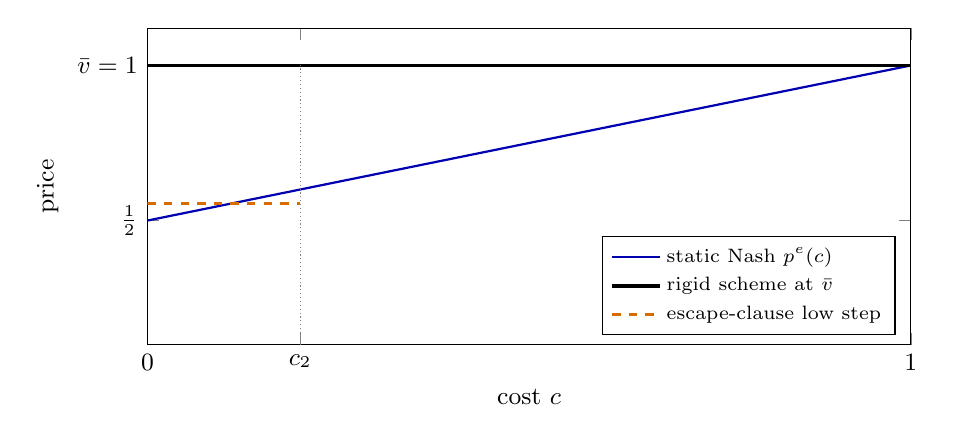
\begin{tikzpicture}
\begin{axis}[width=0.93\linewidth, height=5.6cm, xmin=0, xmax=1, ymin=0.1, ymax=1.12,
  xlabel={cost $c$}, ylabel={price}, xtick={0,0.2,1}, xticklabels={$0$,$c_2$,$1$},
  ytick={0.5,1}, yticklabels={$\frac{1}{2}$,$\bar v = 1$},
  legend style={font=\scriptsize, at={(0.98,0.03)}, anchor=south east}, legend cell align=left,
  tick label style={font=\small}, label style={font=\small}]
\addplot[blue!70!black, thick, domain=0:1, samples=2] {(1+x)/2};
\addlegendentry{static Nash $p^e(c)$}
\addplot[black, very thick, domain=0:1, samples=2] {1};
\addlegendentry{rigid scheme at $\bar v$}
\addplot[orange!85!black, very thick, dashed] coordinates {(0,0.5556) (0.2,0.5556)};
\addlegendentry{escape-clause low step}
\addplot[gray, densely dotted, forget plot] coordinates {(0.2,0.1) (0.2,1)};
\end{axis}
\end{tikzpicture}
\caption{Inelastic demand}
\end{subfigure}\hfill
\begin{subfigure}[b]{0.48\textwidth}
\centering
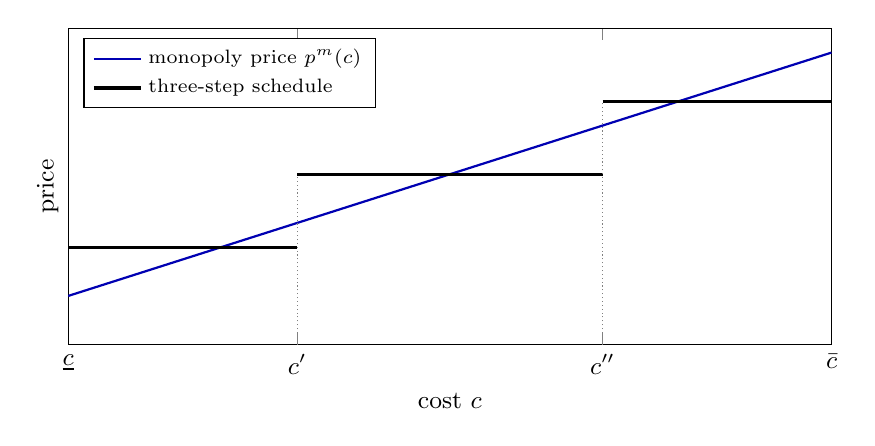
\begin{tikzpicture}
\begin{axis}[width=0.93\linewidth, height=5.6cm, xmin=0, xmax=1, ymin=0.4, ymax=1.05,
  xlabel={cost $c$}, ylabel={price}, xtick={0,0.3,0.7,1}, xticklabels={$\underline c$,$c'$,$c''$,$\bar c$},
  ytick=\empty,
  legend style={font=\scriptsize, at={(0.02,0.97)}, anchor=north west}, legend cell align=left,
  tick label style={font=\small}, label style={font=\small}]
\addplot[blue!70!black, thick, domain=0:1, samples=2] {(1+x)/2};
\addlegendentry{monopoly price $p^m(c)$}
\addplot[black, very thick] coordinates {(0,0.6) (0.3,0.6)};
\addlegendentry{three-step schedule}
\addplot[black, very thick, forget plot] coordinates {(0.3,0.75) (0.7,0.75)};
\addplot[black, very thick, forget plot] coordinates {(0.7,0.9) (1,0.9)};
\addplot[gray, densely dotted, forget plot] coordinates {(0.3,0.4) (0.3,0.75)};
\addplot[gray, densely dotted, forget plot] coordinates {(0.7,0.4) (0.7,0.9)};
\end{axis}
\end{tikzpicture}
\caption{Downward-sloping demand (schematic)}
\end{subfigure}
\caption{Collusive pricing schedules with private costs. Panel (a): two firms, costs uniform on $[0,1]$, reservation
value $\bar v = 1$. The static Nash schedule is $p^e(c) = \frac{1 + c}{2}$. The rigid scheme charges $\bar v$, which
is also the monopoly price, for every cost. A two-step escape-clause scheme charges $\bar v$ above the break point
$c_2$ and a low price on $[0, c_2)$ that keeps type $c_2$ indifferent (here $c_2 = 0.2$ and the low price is $0.556$).
In this uniform example the escape clause is not an equilibrium for $\delta < \delta^*$ (\cref{prop:12-abs-escape}),
so the panel only shows its shape. Panel (b): a three-step schedule. The bottom step lies below the monopoly price of
its highest type $c'$, and the top step lies above the monopoly price of its lowest type $c''$, as
\cref{prop:12-abs-downward}(ii) requires.}\label{fig:12-abs-schedules}
\end{figure}

\subsection{Impatient firms}\label{sec:12-abs-impatient}

Return to inelastic demand and suppose firms are not patient enough to make the off-schedule constraints slack.
After an off-schedule deviation, firms move to a war continuation value $w \in \mathcal V$, for example the worst SPPE
value or reversion to static Nash forever. Its per-period equivalent $\pi^w = (1 - \delta)w$ satisfies (ABS (7), p.~33)
\begin{equation}\label{eq:12-abs-piw}
0 \le \pi^w < \frac{1}{N}\pi(\bar v, \E c) .
\end{equation}
The first inequality holds in any SPPE. The second says that the war is a punishment relative to rigid collusion.
Here $\pi(\bar v, \E c) = \bar v - \E c$ is the expected profit from serving the whole market at $\bar v$.

\begin{proposition}[The threshold discount factor]\label{prop:12-abs-critical}
Let demand be inelastic. A stationary rigid scheme with price $p^r \in [\underline c, \bar v]$ and war value
$\pi^w$ satisfies the off-schedule constraints if and only if both
\begin{equation}\label{eq:12-abs-offschedule}
\frac{N - 1}{N}\,\pi(p^r, \underline c) \;\le\; \frac{\delta}{1 - \delta}\Bigl[\frac{1}{N}\pi(p^r, \E c) - \pi^w\Bigr]
\end{equation}
and
\begin{equation}\label{eq:12-abs-offschedule-high}
\frac{1}{N}\,(\bar c - p^r) \;\le\; \frac{\delta}{1 - \delta}\Bigl[\frac{1}{N}\pi(p^r, \E c) - \pi^w\Bigr]
\end{equation}
hold. If $p^r \ge \bar c$, \eqref{eq:12-abs-offschedule} implies \eqref{eq:12-abs-offschedule-high}. At
$p^r = \bar v$ the scheme therefore satisfies the off-schedule constraints if and only if $\delta \ge \delta^*$, where
\begin{equation}\label{eq:12-abs-deltastar}
\delta^* = \frac{(N - 1)\pi(\bar v, \underline c)}{(N - 1)\pi(\bar v, \underline c) + \pi(\bar v, \E c) - N\pi^w}
\;\in\;\Bigl(\frac{N - 1}{N},\, 1\Bigr).
\end{equation}
If $\delta < \delta^*$, no stationary rigid scheme at any price $p^r \le \bar v$ satisfies \eqref{eq:12-abs-offschedule},
so none satisfies the off-schedule constraints.
\end{proposition}

\begin{proof}
\emph{The constraints.} Under a rigid scheme a firm of type $c$ that undercuts $p^r$ slightly wins the whole market
instead of the share $\frac{1}{N}$. Its current gain is $\frac{N - 1}{N}\pi(p^r, c)$, which is largest for the
lowest type, since $\pi(p^r, c) = p^r - c$. A larger cut only lowers the price it receives. The deviation is
off-schedule, so the continuation drops from the collusive value, worth $\frac{1}{N}\pi(p^r, \E c)$ per period, to
the war, worth $\pi^w$ per period. The loss from the next period on is
$L \equiv \frac{\delta}{1 - \delta}[\frac{1}{N}\pi(p^r, \E c) - \pi^w]$. A type $c$ that raises its price above $p^r$
sells nothing. It earns zero today instead of $\frac{1}{N}(p^r - c)$, which is negative when $c > p^r$. Its current
gain is $\frac{1}{N}(c - p^r)$, which is largest for type $\bar c$, and it faces the same loss $L$. The binding
constraints are thus those of type $\underline c$ against a cut and of type $\bar c$ against a rise, which are
\eqref{eq:12-abs-offschedule} and \eqref{eq:12-abs-offschedule-high}. If $p^r \ge \bar c$, the left side of
\eqref{eq:12-abs-offschedule-high} is at most zero, while \eqref{eq:12-abs-offschedule} gives $L \ge 0$. Then
\eqref{eq:12-abs-offschedule} implies \eqref{eq:12-abs-offschedule-high}. \Cref{asm:12-abs} gives
$\bar v \ge \bar c$, so only \eqref{eq:12-abs-offschedule} matters at $p^r = \bar v$.

\emph{The threshold.} Let $a = (N - 1)\pi(\bar v, \underline c)$ and $b = \pi(\bar v, \E c) - N\pi^w$, which is
positive by \eqref{eq:12-abs-piw}. Multiply \eqref{eq:12-abs-offschedule} at $p^r = \bar v$ by $N(1 - \delta)$:
\begin{equation*}
(1 - \delta)a \le \delta b
\quad\Longleftrightarrow\quad
a \le \delta(a + b)
\quad\Longleftrightarrow\quad
\delta \ge \frac{a}{a + b} = \delta^* .
\end{equation*}
Since $b > 0$, $\delta^* < 1$. Moreover $\delta^* > \frac{N - 1}{N}$ if and only if $(N - 1)(a + b) < Na$, that is,
$(N - 1)b < a$, or $\pi(\bar v, \E c) - N\pi^w < \pi(\bar v, \underline c)$. This holds because
$\pi(\bar v, \underline c) > \pi(\bar v, \E c)$ and $\pi^w \ge 0$.

\emph{Lower rigid prices.} Both sides of \eqref{eq:12-abs-offschedule} are affine in $p^r$, with slopes
$\frac{N - 1}{N}$ on the left and $\frac{\delta}{(1 - \delta)N}$ on the right. If $\frac{N - 1}{N} < \delta < \delta^*$,
the right side rises faster, so the gap between the right and left sides increases in $p^r$. It is negative at
$p^r = \bar v$ and hence negative at every lower $p^r$. If $\delta \le \frac{N - 1}{N}$, the gap is non-increasing in
$p^r$, so the best case is $p^r = \underline c$. There the left side is zero and the right side is negative, since
$\pi(\underline c, \E c) = \underline c - \E c < 0$. In both cases \eqref{eq:12-abs-offschedule} fails (p.~52).
\end{proof}

ABS state \eqref{eq:12-abs-offschedule} as a necessary condition (p.~34). Constraints against price increases that
avoid a loss appear only in footnotes to later proofs (p.~53, footnote~45, and p.~54, footnote~46). In the second
the top price is $\bar v$, and they hold. They matter only for rigid prices below $\bar c$, where \eqref{eq:12-abs-offschedule} alone need not be
sufficient.

ABS extend the last statement to nonstationary schemes. If $\delta < \delta^*$, no SPPE has a rigid price in every
period (ABS Proposition 15, pp.~34 and 52--53). The reason is that the highest rigid price on the path would be
easier to sustain if it were kept forever. Combining the result with \cref{prop:12-abs-rigid}, if $F$ is log-concave and
$\delta \ge \delta^*$, the optimal SPPE has a rigid price at $\bar v$ (ABS Corollary 16, p.~35).

\begin{example}[Cost shocks make collusion harder]\label{ex:12-abs-uniform}
Let $N = 2$, costs uniform on $[0,1]$, $\bar v = 1$, and Nash reversion after an off-schedule deviation (p.~35). By
\cref{ex:12-abs-static-uniform}, $\pi^w = \frac{1}{6}$. Also $\pi(1, 0) = 1$ and $\pi(1, \E c) = \frac{1}{2}$. By
\eqref{eq:12-abs-deltastar},
\begin{equation*}
\delta^* = \frac{1}{1 + \frac{1}{2} - \frac{2}{6}} = \frac{1}{\frac{7}{6}} = \frac{6}{7} \approx 0.857 .
\end{equation*}
Without cost shocks, collusion at a price above a common cost needs only $\delta \ge \frac{1}{2}$ (\cref{prop:12-bertrand}).
The same computation for $N$ firms uses $\pi^w = \frac{1}{N(N + 1)}$ and gives
\begin{equation*}
\delta^*(N) = \frac{N - 1}{(N - 1) + \frac{1}{2} - \frac{1}{N + 1}} = \frac{2(N + 1)}{2N + 3},
\end{equation*}
so $\delta^*(3) = \frac{8}{9}$ and $\delta^*(4) = \frac{10}{11}$, against $\frac{2}{3}$ and $\frac{3}{4}$ without
cost shocks. (This general formula is our own computation. It simplifies because the denominator equals
$\frac{(2N + 3)(N - 1)}{2(N + 1)}$.)
\end{example}

The benchmark $\frac{N - 1}{N}$ is the value of \eqref{eq:12-abs-deltastar} when $\underline c = \E c$ and
$\pi^w = 0$. Cost fluctuations raise the required patience because the scheme must survive the period in which a firm
draws a cost far below the one it expects in the future (p.~35). This holds even if the punishment drives profits to
zero, and the threshold rises further when the punishment is milder. The result fits the common view that collusion is
harder when costs vary across firms and over time \citep[p.~205]{Scherer1980}.

\begin{proposition}[No wars for impatient firms]\label{prop:12-abs-impatient-nowars}
Let demand be inelastic, and let $F$ and $\delta$ be arbitrary. Consider an SPPE with schedule $p$ and continuation
function $v$, and let $z \equiv \sup_{c'}\E_{-i}v(p(c'), \mathbf p_{-i})$. Suppose that
$\E_{-i}v(p(c), \mathbf p_{-i}) < z$ for some $c$, and that a mild regularity condition holds at the top step. Then
there is an SPPE with the same expected payoff in which the continuation value equals $z$ after every on-schedule
price (ABS Proposition 17, p.~37).
\end{proposition}

The proof compares off-schedule constraints. Let $c_k$ be the lowest type on a flat step. With war continuation $w$,
this type's constraint in the original scheme is (ABS (11), p.~53)
\begin{equation*}
\pi\bigl(p(c_k), c_k\bigr)\bigl[(1 - F(c_k))^{N-1} - M(c_k; p)\bigr] \le \delta z - \mathcal T(c_k) - \delta w .
\end{equation*}
Here $\mathcal T(c_k) = \delta[z - \E_{-i}v(p(c_k), \mathbf p_{-i})]$, and the bracket on the left is the gain in
the probability of winning from a slight undercut. The no-war alternative of \cref{lem:12-abs-nowar-equiv} has the same
allocation and a price $\tilde p(c_k) < p(c_k)$ wherever $\mathcal T(c_k) > 0$. Its constraint is (ABS (12))
\begin{equation*}
\pi\bigl(\tilde p(c_k), c_k\bigr)\bigl[(1 - F(c_k))^{N-1} - M(c_k; p)\bigr] \le \delta z - \delta w .
\end{equation*}
The left side is smaller and the right side larger. Moving profit from the present (a lower price today) to the future
(no war tomorrow) reduces the temptation to cheat and raises the value of cooperation at the same time. Wars are thus
doubly harmful for impatient firms with inelastic demand. With downward-sloping demand a war on a step can still help
by relaxing the constraints of types on lower steps (pp.~37--38).

\casehead{An escape clause}
Impatient firms cannot keep a rigid price, but they may support a two-step scheme with a high price $\bar v$ and a
lower price for rare low-cost draws.

\begin{proposition}[Escape clause]\label{prop:12-abs-escape}
Let demand be inelastic and $N = 2$. If
\begin{equation}\label{eq:12-abs-escape}
f(\underline c) < \frac{\frac{1}{2}\pi(\bar v, \E c) - \pi^w}{\pi(\bar v, \underline c)\,\pi^w},
\end{equation}
there is $\delta^\circ < \delta^*$ such that, for every $\delta \in (\delta^\circ, \delta^*)$, a two-step schedule with
prices $p_2 = \bar v > p_1$ and a break point $c_2 \in (\underline c, \bar c)$ is an SPPE (ABS Proposition 18,
p.~39).
\end{proposition}

The working paper prints the denominator of \eqref{eq:12-abs-escape} as $\bar v\,\pi^w$. The two agree when
$\underline c = 0$, as in all its examples. For general $\underline c$ the slope comparison in its proof gives
$\pi(\bar v, \underline c)\,\pi^w$, as we show below. With $\underline c > 0$ the printed condition is a stronger
sufficient condition.

We do not reproduce the whole existence proof (pp.~53--55), which is a continuity argument. At $\delta = \delta^*$ and
$c_2 = \underline c$ the two-step scheme is the rigid one, and its off-schedule constraints bind. Under
\eqref{eq:12-abs-escape}, raising $c_2$ slightly makes these constraints slack. The slack lets a two-step scheme
survive for $\delta$ slightly below $\delta^*$. The binding constraint for small $c_2$ is that of type $c_2$
undercutting $\bar v$. Its current gain is $\Omega(c_2) = \frac{1}{2}\pi(\bar v, c_2)[1 - F(c_2)]$. Let $W(c_2)$
be the expected per-period profit of the two-step scheme minus $\pi^w$, so the loss from a war is
$\frac{\delta}{1-\delta}W(c_2)$. Differentiating the expressions for $\Omega$ and $W$ on p.~54 of ABS at
$c_2 = \underline c$ gives
\begin{equation*}
\Omega'(\underline c) = -\frac{1}{2}\bigl[1 + f(\underline c)\,\pi(\bar v, \underline c)\bigr],
\qquad
W'(\underline c) = -\frac{1}{2}f(\underline c)\,\pi(\bar v, \E c) .
\end{equation*}
The constraint gains slack as $c_2$ rises from $\underline c$ if $\frac{\delta^*}{1-\delta^*}W'(\underline c) >
\Omega'(\underline c)$. With $N = 2$, \eqref{eq:12-abs-deltastar} gives
$\frac{\delta^*}{1-\delta^*} = \frac{\pi(\bar v, \underline c)}{\pi(\bar v, \E c) - 2\pi^w}$, and the inequality
rearranges to \eqref{eq:12-abs-escape}.

The on-schedule constraint pins down the low price (ABS (13), p.~53). Type $c_2$ must be indifferent between the two
steps. With two firms, a firm on the low step wins unless the rival is also on it, in which case they tie, so
$M_1 = 1 - \frac{F(c_2)}{2}$. A firm on the high step wins half the time when the rival is also high, so
$M_2 = \frac{1 - F(c_2)}{2}$. Indifference, $(p_1 - c_2)M_1 = (\bar v - c_2)M_2$, gives
\begin{equation}\label{eq:12-abs-p1}
p_1 = c_2 + (\bar v - c_2)\,\frac{1 - F(c_2)}{2 - F(c_2)} .
\end{equation}
As $c_2 \to \underline c$, $p_1 \to \frac{\bar v + \underline c}{2}$. With $\underline c$ near zero the low price is
about half the high price, the 50 percent cut that ABS report for their construction with $c_2$ close to $\underline c$
(p.~39, footnote 32). In the uniform example with $c_2 = 0.2$, $p_1 = 0.2 + \frac{0.64}{1.8} = 0.556$
(\cref{fig:12-abs-schedules}).

The escape clause works through two effects (pp.~38--39). The lowest-cost firm now expects more than the share
$\frac{1}{N}$, at a lower price, so its gain from undercutting is smaller. With $c_2$ close to $\underline c$, one can
check from \eqref{eq:12-abs-p1} that the most tempted type becomes the break-point type $c_2$. Its best deviation is
a price just below $\bar v$, and its cost exceeds $\underline c$. Against this, a two-step scheme
earns less than the rigid scheme when $F$ is log-concave, so a deviator also has less to lose. A small density at the
bottom keeps the second effect small, which is what \eqref{eq:12-abs-escape} requires. The condition is restrictive.
For $F(c) = c^\alpha$ on $[0,1]$ it holds when $\alpha > 1$ and fails for $\alpha \le 1$ (p.~39). In the uniform
example the right side of \eqref{eq:12-abs-escape} is $\frac{\frac{1}{4} - \frac{1}{6}}{\frac{1}{6}} = \frac{1}{2} <
1 = f(0)$. There, two-step schemes fail the off-schedule constraint for exactly the same discount factors as the rigid
scheme (pp.~39--40).

The escape clause has an interpretation that matters for reading cartel histories (pp.~39, 47). Collusion among
impatient firms may be marked by occasional, large price cuts by single firms after favorable cost draws, which rivals
do not punish. They are a permitted exception, firm by firm, much as \citet{RotembergSaloner1986} allow prices to
fall when demand is high. In that model, however, all firms adjust together in response to a public shock.

Finally, under log-concavity and a non-decreasing density, an optimal stationary SPPE for impatient firms that beats
Nash has no open interval of strictly increasing prices (ABS Proposition 19, p.~41). It is a step function: partial
rigidity. The analysis is a static mechanism design problem with two unusual features. The participation constraints
depend on the type, and they are endogenous, because the value of the outside option depends on the scheme itself
(pp.~40--42).

\subsection{Asymmetric schemes}\label{sec:12-abs-asymmetric}

Symmetric equilibria allow only wasteful transfers, borne by all firms. Asymmetric perfect public equilibria also let
firms transfer value from one firm to another through the continuation, for example by favoring in future periods a
firm that has sold little (p.~43). ABS illustrate with two simple schemes, using two firms, inelastic demand, uniform
costs on $[0,1]$, $\bar v = 1$ and Nash reversion.

\casehead{Taking turns}
In a \emph{take-turns} scheme the firms alternate in serving the market at $\bar v$. With inelastic demand it offers
no efficiency gain over rigid pricing, since the winner's identity is independent of costs. It needs more patience.
The most tempted firm is one whose turn it is to sit out and which has drawn cost zero. Undercutting gives it
$\pi(1, 0) = 1$ now and the Nash value $\frac{\delta}{1 - \delta}\cdot\frac{1}{6}$ afterward. Conforming gives nothing
now and the expected profit $\frac{1}{2}$ in every other period from the next one on, worth
$\frac{\delta}{1 - \delta^2}\cdot\frac{1}{2}$. The constraint is
\begin{equation*}
\frac{\delta}{2(1 - \delta^2)} \ge 1 + \frac{\delta}{6(1 - \delta)} .
\end{equation*}
Multiply by $6(1 - \delta^2)$ to get $3\delta \ge 6(1 - \delta^2) + \delta(1 + \delta)$, that is,
$5\delta^2 + 2\delta - 6 \ge 0$. The positive root is $\frac{\sqrt{31} - 1}{5} = 0.9135$, above $\delta^* = 0.857$
(p.~44, footnote 38).

\casehead{A two-price scheme}
In the \emph{two-price scheme} $(p^l, \bar v)$, each firm may charge the low price $p^l$ exactly once in every
two-period cycle and $\bar v$ in the other period (p.~44). In the first period of a cycle a firm chooses between the
sequences $(p^l, \bar v)$ and $(\bar v, p^l)$. Using the low price now forfeits it tomorrow, when the firm's cost may
be lower, so only firms with low current costs take it. Types below a cutoff $c^\dagger$ choose $(p^l, \bar v)$. (ABS
write $\theta^*$ for the cutoff.)
Indifference of type $c^\dagger$ when the rival uses the same cutoff gives (ABS (10), p.~45)
\begin{multline*}
F(c^\dagger)\,\frac{\pi(p^l, c^\dagger) + \delta\pi(\bar v, \E c)}{2} + [1 - F(c^\dagger)]\,\pi(p^l, c^\dagger) \\
= F(c^\dagger)\,\delta\pi(p^l, \E c) + [1 - F(c^\dagger)]\,\frac{\pi(\bar v, c^\dagger) + \delta\pi(p^l, \E c)}{2} .
\end{multline*}
The left side is the expected two-period profit from using the low price first, and the right side from using it
second.\footnote{The equation printed as (10) in the working paper (p.~45) has no factor $\delta$ on the term
$\pi(\bar v, \E c)$ in its top line. We restore it, because the second-period profit must be discounted like every
other second-period term. With the factor restored, the approximation $c^\dagger \approx \frac{2 - \delta}{2}$ that ABS
state follows, and without it the approximation does not hold.} With $p^l$ close to $\bar v = 1$ and uniform costs, let $x = c^\dagger = F(c^\dagger)$. The difference between
the two sides reduces to $\frac{1 - x}{2} - \frac{\delta}{4}$, so $c^\dagger \approx \frac{2 - \delta}{2}$, which lies in
$(\frac{1}{2}, 1]$ (p.~45). A firm with cost below $c^\dagger$ uses its low price in the first period, so some sorting
occurs at almost no price distortion, and the scheme beats rigid pricing. Sorting rises with $\delta$, and as
$\delta \to 1$ the cutoff tends to the median cost. The scheme still needs patience, $\delta \ge \delta^{**} \approx
0.88$, above $\delta^*$ though below the take-turns threshold (p.~46, footnote 41). Its novel prediction is that a
firm's market share is negatively correlated over time. ABS suggest that such schemes suit small groups of firms that
track each other's sales and communicate explicitly. \citet{AtheyBagwell2001} study optimal asymmetric collusion with
communication about costs.

\subsection{Testable implications, limitations and contribution}\label{sec:12-abs-assessment}

\Cref{tab:12-abs-results} collects the main results. They yield several predictions (pp.~46--48). Collusive prices
are rigid with respect to firm-specific, privately observed cost shocks. They respond to public cost shocks, such as
a change in a common wholesale price, because the whole scheme can be re-tailored to a public change. Prices are more
rigid in concentrated, collusive industries. Optimal collusion among patient firms involves no price wars, unlike
\cref{sec:12-gp-original}. Impatient cartels may show occasional large price cuts by single firms that rivals ignore.
ABS offer this as an alternative reading of apparent unpunished cheating, an issue raised for the Sugar Institute by
\citet{GenesoveMullin2001}, whose working-paper version ABS cite (p.~47, footnote 43). ABS also combine private costs
with the persistent demand phases of \citet{BagwellStaiger1997}. They conjecture that off-schedule constraints are
easier to meet in booms when growth rates are positively correlated, so prices may be more rigid in booms (p.~48).

\begin{table}[htbp]
\centering
\caption{Optimal symmetric collusion with private costs}\label{tab:12-abs-results}
\begin{tabularx}{\textwidth}{@{}l>{\raggedright\arraybackslash}X>{\raggedright\arraybackslash}X@{}}
\toprule
 & Inelastic demand & Downward-sloping demand \\
\midrule
Fully sorting schemes & Best is repeated static Nash (\cref{prop:12-abs-fullsort}) & Best is repeated static Nash, and all others are strictly worse (\cref{prop:12-abs-downward}(i)) \\
Patient firms: wars & Never needed (\cref{prop:12-abs-nowars}) & Never at the top or bottom step, possible only on intermediate steps (\cref{prop:12-abs-downward}(ii) and (iii)) \\
Patient firms: prices & Rigid at $\bar v$ if $F$ is log-concave (\cref{prop:12-abs-rigid}) & Rigid at the bottom, single rigid price if demand is inelastic enough and $F$ log-concave (\cref{prop:12-abs-downward}(iv)) \\
Impatient firms & Rigid price at $\bar v$ if and only if $\delta \ge \delta^*$ (\cref{prop:12-abs-critical}), no wars (\cref{prop:12-abs-impatient-nowars}), escape clause for small $f(\underline c)$ (\cref{prop:12-abs-escape}), step functions & Wars on a step may relax lower types' constraints \\
\bottomrule
\end{tabularx}

\smallskip
\begin{minipage}{0.95\textwidth}
\footnotesize Notes: SPPE, costs \iid\ across firms and periods. Source: \citet{AtheyBagwellSanchirico2004},
working-paper version, Propositions 8 to 19.
\end{minipage}
\end{table}

\casehead{Limitations}
The analysis restricts attention to symmetric equilibria, which ABS defend on three grounds (pp.~6--7). Under many
conditions the optimal SPPE is stationary and simple. Symmetric schemes capture the fear of industry-wide breakdowns,
and they are the only option when the identity of the seller is not observed. Asymmetric schemes do better when firms
are patient and sophisticated. Costs are \iid\ over time. With persistent costs a firm's current price reveals
information about its future costs, which changes the incentive problem. \citet{AtheyBagwell2008} study that case.
The clean results rely on inelastic demand, and with downward-sloping demand the characterization is partial. There
is no communication in the symmetric analysis. \citet[p.~2431]{HarringtonSkrzypacz2011} contrast their setting with
the asymmetric extension of this analysis with communication \citep{AtheyBagwell2001,AtheyBagwell2008}. There, prices
are public and firms report private costs so that the low-cost firm can be given more market share. In the model of
Harrington and Skrzypacz, prices and sales are private, and firms report sales so that the cartel can monitor
compliance (\cref{sec:12-hs}).

\casehead{Contribution}
ABS identify a basic trade-off for colluding firms with private information. Sorting by cost buys productive
efficiency at an informational cost, paid in distorted prices or in wars. Rigidity removes the informational cost at
the price of efficiency. They show that rigidity usually wins and that optimal collusion rarely needs wars, which gives
an equilibrium foundation to the old association between collusion and rigid prices. Methodologically, they connect
repeated games with hidden information to static mechanism design, with restricted transfers and endogenous,
type-dependent participation constraints. \Cref{sec:12-cartels} turns to the way real cartels use communication to
relax these constraints.
